
\begin{center}
\textit{Based on a provided toolbox for solving the travelling salesman problem (TSP), some parameter tuning with the default operators, selection methods, ... was performed. Then, new tour representations and accompanying operators were implemented. Local heuristics, other selection methods, the island model, adaptive parameter tuning and a seeding technique were also experimented with. The results are outlined below. Pointers to relevant source code files are provided next to section headings (all code is written in \texttt{MATLAB}).}
\end{center}

\fakesection{Existing Genetic Algorithm}{\hfill\small\texttt{/experiments/*.m}}

To get an initial feel for what may or may not be worth it, 375 configurations (table \ref{tab:par1}) were experimented with for a total of 15,000 runs. This made it possible to draw some initial conclusions and perform some increasingly targeted experiments afterwards. All of the experiments outlined throughout this report were automated, with occasional use of parallelism (using \texttt{MATLAB}'s parallel computing toolbox).

\begin{table}[h]
\centering
\begin{tabular}{c|c|c|c}
\textit{Population Size} & \textit{Crossover Rate (\%)} & \textit{Mutation Rate (\%)} & \textit{Elitism (\%)} \\\hline 
[150,300,600] & [10,25,50,75,95] & [5,25,50,75,95] & [1,5,10]
\end{tabular}
\caption{Parameter ranges for the initial experiments. Each configuration was run 10 times on 4 different datasets (with 25, 41, 70 and 127 cities). No stopping criterion was applied, and each run lasted 250 generations. For all configurations with population size set to 150 runs with 500 generations were also experimented with. Results are visualised in tables \ref{tab:res1} to \ref{tab:res5}.}
\label{tab:par1}
\end{table}

\noindent After selecting 4 datasets (with an increasing amount of cities) each of the resulting algorithms were ran 10 times. The resulting (best, average and worst) tour lengths and runtimes were recorded and averaged. The best tour found by each was also recorded, since the very point of the travelling salesman problem is to find the smallest possible tour. Diversity of solutions is only of indirect benefit as it increases the probability of reaching a global optimum. The minimum tour length found by every configuration is visualised in tables \ref{tab:res1} to \ref{tab:res5}. It is calibrated against the minimum and maximum found by any of the 375 configurations (darker cells in the table indicate better solutions).\\

\par\noindent Aside from the obvious conclusion that the first benchmark is a tad too easy to resolve, two observations could be made ; larger population sizes improved results and lead to longer runtimes, and setting the rate of elitism too low is contra-productive. The first is not surprising since a larger population may increase diversity and the probability of finding a better local (or even global) minimum. At its worst it introduces redundancy and needlessly increases runtime. As for the second conclusion, retaining a reasonable proportion of the best individuals looks like a safe bet. Higher levels of elitism (> 10\%) proved to be somewhat less fruitful. While better individuals may appear attractive to the greedy, some of them probably represent second-hand solutions (those that haven't been mutated to one of the better individuals yet, or better individuals that have been unsuccessfully mutated) that may safely be disregarded.\\

\par\noindent The effect of population size was suspected - at least partially - to be due to increased speed of convergence. This was tested by running all configurations with population size of 150 for a larger number of generations which confirmed the suspicion (table \ref{tab:res4}). Therefor, future experiments use a reasonably large population size (300), fair rate of elitism (5-20\%) and an appropriate stopping criterion (or the number of generations is set reasonably high).\\

\par\noindent One slightly more surprising result is that higher mutation - and crossover rates appeared to worsen results. High rates of mutation are too disruptive and the default crossover operator (alternating edges) preserves few edges from the parent. In subsequent experiments, only rates of 5\% and 95\% were abandoned.\\

\par\noindent It can be noted that just 10 runs and 250 generations is hardly enough (from a statistical point of view). However, only soft conclusions were drawn and limited computing power and time was available. Subsequent experiments were usually run 30 times per configuration and tend to make use of a stopping criterion (in combination with a high maximum number of generations) to avoid prematurely stopping a run. While it would be preferable no non-parametric tests were applied. Additionally, while the number of values that were tried per parameter isn't very high, testing out more values would make for a combinatorial explosion. So only a small part of the utility landscape was explored. For a better analysis iterative methods could be used rather than this basic GENERATE-and-TEST approach.

\fakesection{Stopping Criterion}{\hfill\small\texttt{/stop\_criteria/*.m}}

%Implement a stopping criterion that avoids that rather useless iterations (generations) are computed.
%\begin{enumerate}
%\item	 Stopping criterion \& explain why you selected this criterion
%\item Test results (incl.\ performance criteria and parameter settings)
%\item Discussion of test results
%\end{enumerate}

The following efficiency function $E$ is used to calculate the algorithm's efficiency after each generation:
\begin{equation}
    E(T) = \frac{1}{T} \sum_{t=0}^T F_i
\end{equation}
where $T$ is the index of the current generation and $F_i$ the best fitness value of generation $i$. This efficiency function basically calculates the average best fitness over all generations. Since the total distance is used as the fitness of an individual and the goal is to minimize this distance, $E(t)$ is a monotonically decreasing function (assuming elitism is used).\\
\newline
The stopping criterion keeps track of the efficiency of the algorithm. When the relative standard deviation of the last $W$ efficiency values (window) drops below a certain percentage $\Delta$, the algorithm stops. $\Delta$ was chosen to be 0.5\%. This stop criterion seems suitable, since the goal is to avoid useless generations where little to no improvement of the solution happens.\\
\newline
The window size $W$, being the only parameter not yet fixed, influences the quality of the solution and the convergence speed (in generations) of the algorithm. A small $W$ will make the algorithm terminate sooner, possibly missing out on better solutions and decreasing the solution quality. A large $W$ will make the algorithm terminate later, possibly increasing the solution quality but also allowing more useless generations.\\
\newline
An optimal value for $W$ was determined. The algorithm was run 20 times on each small benchmark (\texttt{rondrit<...>, belgiumtour, xqf131}) with 500 generations (induvuduals = 50, elitism = 0.05, P\_cross = 0.7, P\_mut = 0.55, crossover = xalt edges, representation = adjacency, mutation = simple inversion, parent selection = linear rank, survivor selection = fitness based). \\
For each run, the evolution of the efficiency was observed to see what the longest streak without change greater than $\Delta$ was (excluding the last streak until termination of the run). The average streak was 30 with a standard deviation of 35.\\
\newline
Two window sizes were considered, namely 30 (the average) and 66 (the sum of the average and standard deviation plus one). The same setup as above was run, but with the stop criterion activated. Each time the stop criterion was met, the generation and fitness value were saved, but the run completed the full 500 generations, so the difference in quality could be observed. The results are shown in the table \ref{tab:window30} and table \ref{tab:window66} below.\\

\begin{table}[ht!]
    \centering
    \begin{tabular}{ | l || l | l | l || l | l | l || l | }
    \hline
     & \multicolumn{3}{|c|}{No stop criterion} & \multicolumn{3}{|c|}{Stop criterion (W = 30)} & \\
    \hline
	Route & \# gen & avg best & std best & \# gen & avg best & std best & quality decrease(\%) \\ \hline
	rondrit016 & 500 & 1484.877 & 12.547 & 142.35 & 1514.335 & 33.365 & 1.945 \\ \hline
	rondrit018 & 500 & 1202.425 & 39.508 & 199.7 & 1233.302 & 69.093 & 2.504 \\ \hline
	rondrit023 & 500 & 832.020 & 26.397 & 280.650 & 870.636 & 45.998 & 4.435 \\ \hline
	rondrit025 & 500 & 41.407 & 1.272 & 311.75 & 43.251 & 2.112 & 4.262 \\ \hline
	rondrit048 & 500 & 4677.841 & 262.778 & 423.45 & 4938.954 & 472.199 & 5.287 \\ \hline
	rondrit050 & 500 & 8.754 & 0.521 & 414.55 & 9.249 & 0.965 & 5.3539 \\ \hline
	rondrit051 & 500 & 625.062 & 21.971 & 373.75 & 672.535 & 57.825 & 7.059 \\ \hline
	rondrit067 & 500 & 4241.510 & 290.263 & 396.95 & 4649.488 & 626.395 & 8.775 \\ \hline
	rondrit070 & 500 & 1334.162 & 58.237 & 422.1 & 1420.047 & 121.276 & 6.048 \\ \hline
	rondrit100 & 500 & 21.866 & 0.796 & 356.85 & 24.537 & 1.531 & 10.887 \\ \hline
	rondrit127 & 500 & 317.718 & 10.040 & 251.45 & 371.896 & 29.412 & 14.568 \\ \hline
	belgiumtour & 500 & 877.212 & 45.774 & 391.25 & 926.090 & 82.716 & 5.278 \\ \hline
	xqf131 & 500 & 1943.598 & 76.138 & 339.4 & 2192.587 & 156.261 & 11.356 \\ \hline
    \end{tabular}
    \caption{Each benchmark solved 20 times with a a max generation of 500. This table shows the amount of generations, average best fitness and standard deviation at the moment the stop criterion (W = 30) fired and the moment the algorithm finished the max generation. The quality is compared.}
    \label{tab:window30}
\end{table}

\begin{table}[ht!]
    \centering
    \begin{tabular}{ | l || l | l | l || l | l | l || l | }
    \hline
     & \multicolumn{3}{|c|}{No stop criterion} & \multicolumn{3}{|c|}{Stop criterion (W = 66)} & \\
    \hline
	Route & \# gen & avg best & std best & \# gen & avg best & std best & quality decrease(\%) \\ \hline
	rondrit016 & 500 & 1497.412 & 20.705 & 237.55 & 1514.721 & 29.710 & 1.143 \  \\ \hline
	rondrit018 & 500 & 1184.392 & 23.386 & 339.75 & 1188.051 & 32.231 & 0.308 \  \\ \hline
	rondrit023 & 500 & 841.468 & 27.097 & 477.3 & 842.007 & 26.667 & 6.398E-2 \  \\ \hline
	rondrit025 & 500 & 40.990 & 0.719 & 492.8 & 41.273 & 1.328 & 0.687 \  \\ \hline
	rondrit048 & 500 & 4746.863 & 265.478 & 500 & 4746.863 & 265.478 & 0 \  \\ \hline
	rondrit050 & 500 & 8.806 & 0.420 & 500 & 8.806 & 0.420 & 0 \  \\ \hline
	rondrit051 & 500 & 608.155 & 29.390 & 500 & 608.155 & 29.390 & 0 \  \\ \hline
	rondrit067 & 500 & 4271.311 & 268.417 & 500 & 4271.311 & 268.417 & 0 \  \\ \hline
	rondrit070 & 500 & 1321.352 & 81.164 & 500 & 1321.352 & 81.164 & 0 \  \\ \hline
	rondrit100 & 500 & 21.797 & 0.651 & 500 & 21.797 & 0.651 & 0 \  \\ \hline
	rondrit127 & 500 & 315.640 & 11.969 & 500 & 315.640 & 11.969 & 0 \  \\ \hline
	belgiumtour & 500 & 886.170 & 57.198 & 500 & 886.170 & 57.198 & 0 \  \\ \hline
	xqf131 & 500 & 1944.138 & 84.712 & 500 & 1944.138 & 84.713 & 0 \  \\ \hline
    \end{tabular}
    \caption{Each benchmark solved 20 times with a a max generation of 500. This table shows the amount of generations, average best fitness and standard deviation at the moment the stop criterion (W = 66) fired and the moment the algorithm finished the max generation. The quality is compared.}
    \label{tab:window66}
\end{table}

\noindent As expected, the smaller window size ($W = 30$) results in faster termination and worse quality, the bigger window size in better solution quality and slower termination. \\
Another interesting observation is the quality decrease in function of the route size (number of cities). These larger routes are more complex and thus the algorithm converges slower. A small window size ($W = 30$) will let the algorithm terminate while the solution is still improving slowly but steadily. A larger window size ($W = 66$) will observe the slow progress and let the algorithm run longer. Taking the window size too large, might result in many generations with too little improvement, though.\\
\newline
These results show that the window size and this type of stop criterion in general, are problem specific. As a result, this criterion is only suitable for applications where only one problem or problems of similar complexity are to be solved.

\fakesection{Other Representation and Appropriate Operators}{\hfill\small\texttt{/crossovers/*.m}, \texttt{/mutations/*.m}}

Aside from the adjacency representation, (at least) four alternative representations can be used. Two of those are binary which were avoided due to previous experiences in constraint programming where the use of binary representations for problems with integer domains is discouraged. They are the binary and matrix representations. The other two alternatives were both implemented. The ordinal representation because it allows for the use of the \textit{`classic'} single-point crossover. The path representation because it is probably the most \textit{`natural'} representation. For the latter a few crossover operators were implemented (inspired by \cite{larraaga} \& \cite{imskhan}). Some of these were mentioned either in Eiben's book or in the course notes ; the \textit{heuristic} - , \textit{partially matched} -, \textit{order} -, \textit{cycle} -, \textit{edge recombination} - and \textit{sequential constructive} crossovers in particular. Operators that weren't mentioned include : 
\begin{itemize}
\item[-] \textit{Heuristic Edge Recombination (HERX)} : equivalent to the edge recombination crossover, but with some hybridisation in that the shortest edge is picked from the edge list of the current city, rather than the edge corresponding to the city with the shortest edge list.
\item[-] \textit{Max Preservative (MPX)} : similar to the partially matched crossover. A subtour of the first parent is selected and remaining cities are \textit{appended} to this sequence in the order that they appear in the other parent. The subtour's length needs to be within a specified interval.
\item[-] \textit{Order Based (OX2)} : a few random cities are selected in a parent. These cities are removed from the other parent and replaced by the same cities, at the same locations, but in the order that they appear in the first parent.
\item[-] \textit{Position Based (POS)} : this one also selects a few random cities but imposes their positions as well, such that the offspring is the same as the first parent with respect to the cities that were selected, after which the remaining cities are added to it in the order that they appear in the other parent.
\item[-] \textit{Unnamed Heuristic (UHX)} : a city is selected randomly. Four edges connected to city are compared, the smallest is picked (if there are edges of equal length, one is picked at random). The city at the other side of this edge becomes the current city and the whole routine is repeated until all cities have been added to the offspring.
\end{itemize}
The following mutation operators were implemented :
\begin{itemize}
\item[-] \textit{Insertion} : a city is selected, removed and inserted at some other (random) point in the tour.
\item[-] \textit{Displacement} : a subtour is selected, removed and inserted at some other point in the tour.
\item[-] \textit{Inversion} : the `simple' inversion was already implemented. It involves picking out two cities and inverting the subtour between them (which is what 2-opt does). Inversion adds to this by subsequently placing it somewhere else (like the displacement operator does).
\item[-] \textit{Scramble} : selects a random subtour and shuffles the cities around. Clearly quite a disruptive operator.
\item[-] \textit{Unnamed} : a hybridised operator, just like its accompanying crossover. A random city is selected and the subtour from this city to the one closest to it is reversed.
\end{itemize}
These operators were selected such that a general idea could be formed about them. Some are clearly less \textit{`respectful`} than others, yet it wasn't entirely clear what to expect aside from what was reported in a fairly limited amount of studies which used other benchmarks. After some manual experiments (within the GUI that was extended for this purpose) further experimentation was done with all crossovers. From the configurations that were trialed before, 9 were selected and each of the crossover operators were tested in conjunction with those parameter values (table \ref{tab:par2}). The results are displayed in figures \ref{fig:rescross1} to \ref{fig:rescross4} (heatmaps might have been a preferable visualisation and can be generated from the \texttt{crossoverlatex} script, but they were a tad less interpretable). The average best tour length was visualised as well but not included in the report, as there was no indication that the shortest tours were a matter of luck.\\

\par\noindent As for the runtimes ; the edge recombination crossovers (both the classical and heuristic one) involve construction of an edge map which makes them the slowest in our list. The sequential crossover is a tad slower too, as is the classic single-point crossover (probably because the associated ordinal representation requires conversion to a path representation upon mutation). It's the latter, \texttt{SCX}, \texttt{HERX} and \texttt{UHX} operators who converge more rapidly. The last three are hybrid which makes this unsurprising.

\begin{table}[h]
\centering
\begin{tabular}{c|c|c|c|c}
\textit{Population Size} & \textit{Crossover Rate (\%)} & \textit{Mutation Rate (\%)} & \textit{Elitism (\%)} & \textit{Generations} \\\hline 
[300] & [25,50,70] & [25,50,70] & [5] & [1000]
\end{tabular}
\caption{Parameter ranges for the experiments on crossover operators. Each configuration was run 10 times on 4 different datasets (with 70, 100, 127 and 131 cities). A stopping criterion was used to avoid useless iterations ; the algorithm stops if the best individual hasn't improved much in the past 100 generations. Results are visualised in figures \ref{fig:rescross1} to \ref{fig:rescross4}.}
\label{tab:par2}
\end{table}

\par\noindent After selection of the 4 more promising crossovers they were tested in combination with all of the 6 remaining mutation operators (all but simple inversion). The results are visualised in figures \ref{fig:resmut1} and \ref{fig:resmut2}. To some extent an assumption is made that the performance of mutation operators can be gauged separately from the crossover operator in the sense that it wasn't tested if the other 9 crossover operators perform better than others when combined with a particular mutation operator. Again, given the multitude of possible combinations some simplification is in order. Ideally a meta-algorithm would be used to automate the parameter tuning.

\begin{table}[H]
\centering
\begin{tabular}{c|c|c|c|c}
\textit{Population Size} & \textit{Crossover Rate (\%)} & \textit{Mutation Rate (\%)} & \textit{Elitism (\%)} & \textit{Generations} \\\hline 
[300] & [50] & [20,40,50,70] & [5] & [1000]
\end{tabular}
\caption{Parameter ranges for the experiments on mutation operators. Each configuration was run for 4 different datasets (with 70, 100, 127 and 131 cities). A stopping criterion was used to avoid useless iterations ; the algorithm stops if the best individual hasn't improved much in the past 100 generations. Results are visualised in figures \ref{fig:resmut1} to \ref{fig:resmut2}.}
\label{tab:par3}
\end{table}

\noindent The insertion, simple inversion and reciprocal exchange mutations appeared to be a safe bet in this limited number of experiments. They're not particularly disruptive in comparison with, say, the scramble and displacement mutation operators. Performance of algorithms didn't differ much between runs ; the results for mean shortest tour length (rather than minimum shortest tour across runs) is about equivalent. Of the four mutation rates that were tested the middle 2 (40\% and 50\%) appeared to be appropriate for future use. The scramble mutation turned out to be the most unpredictable. Mutations can get one out of a local optimum or just improve the value of the best solution found so far, but getting towards the optimum is clearly still not guaranteed.

\fakesection{Local Optimisation}{\hfill\small\texttt{/hybridisation/twoopt.m}, \texttt{/hybridisation/oropt.m}}

In addition to the loop detection heuristic which was already part of the toolbox, two of the more simple heuristics were applied on some of the benchmarks. \textit{Two-opt} and \textit{Or-opt} in particular\footnote{There's some overlap between the \textit{two-opt} operator and the local loop detection so it's somewhat useless to combine both.}. While not as powerful as the Lin-Kernighan heuristic (which even has some efficient implementations), they're easy to implement and provide good results. Their time complexity is $\mathcal{O}(N^2)$ (per tour). The experiments turned out to be fairly uninteresting in that apparently optimal results were found for each of the smaller tours. One of the better crossovers was tested in combination with these heuristics on \texttt{XQF131}. A near-optimal tour was found with just one erroneous sequence in the bottom left corner. The value of the heuristics is visualised more clearly in the experiments at the end of this report.\\

\par\noindent \textit{Or-opt} is a restricted version of \textit{3-opt} in which subtours of length 1, 2 or 3 are displaced. If the resulting tour is shorter it is picked for further processing. While \textit{2-opt} makes the simple inversion mutation redundant, \textit{Or-opt} obviously overlaps with some mutation operators as well. Results obtained with this heuristic were typically inferior to those obtained with \textit{2-opt}.

\fakesection{Benchmark Problems}{}

Tests on benchmarks were run without any local heuristic (results where they \textit{are} activated are visualised at the end of this report). Parameters used are listed in table \ref{tab:bench1}. The results are displayed below.

\begin{figure}[H]
	\centering
%
	\begin{subfigure}[b]{0.45\textwidth}
		\centering
		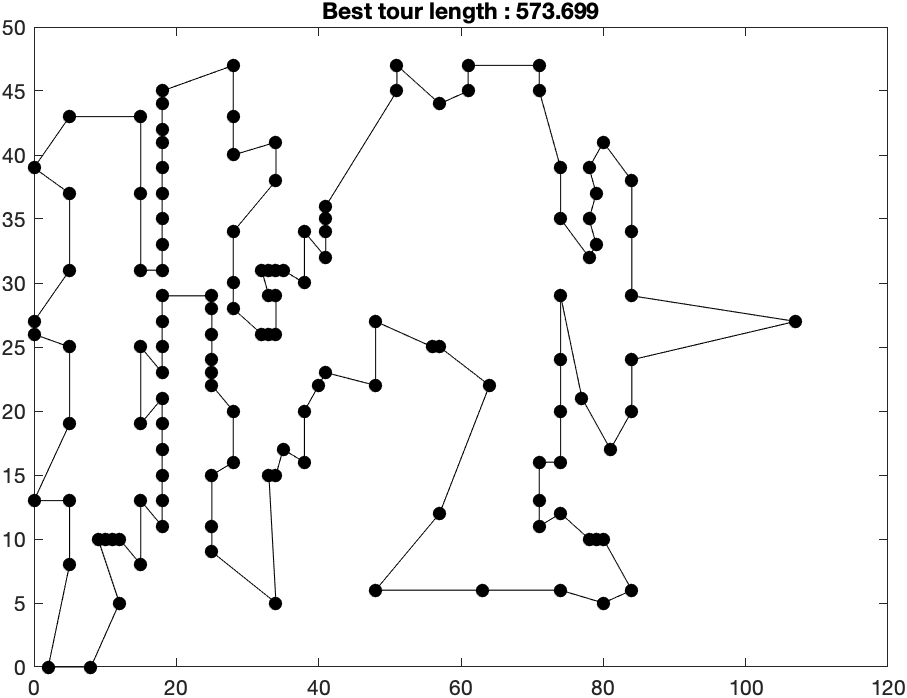
\includegraphics[width=\textwidth]{benchmarks/xqf131.png}
		\caption{\texttt{xqf131}}
    	\end{subfigure}
	\begin{subfigure}[b]{0.45\textwidth}
		\centering
		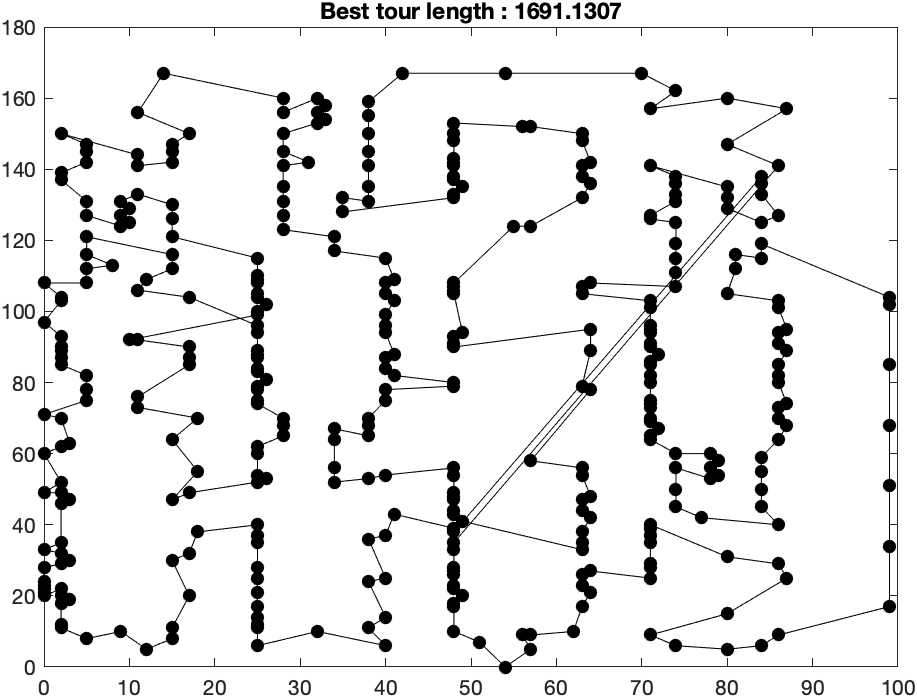
\includegraphics[width=\textwidth]{benchmarks/bcl380.png}
		\caption{\texttt{bcl380}}
    	\end{subfigure}
\end{figure}
\begin{figure}[H]
	\centering
	\begin{subfigure}[b]{0.45\textwidth}
		\centering
		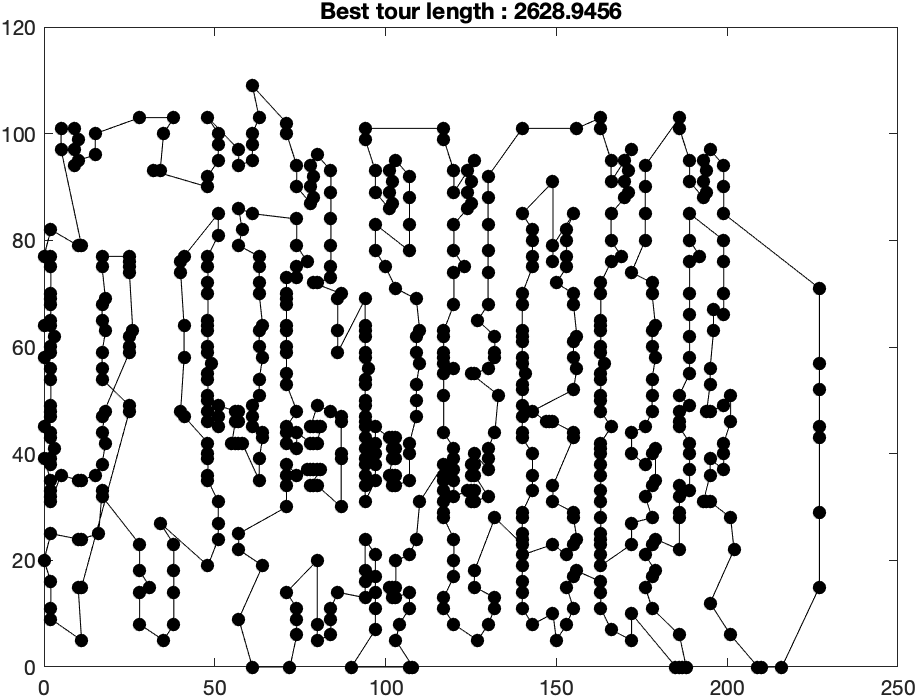
\includegraphics[width=\textwidth]{benchmarks/xql662.png}
		\caption{\texttt{xql662}}
    	\end{subfigure}
	\begin{subfigure}[b]{0.45\textwidth}
		\centering
		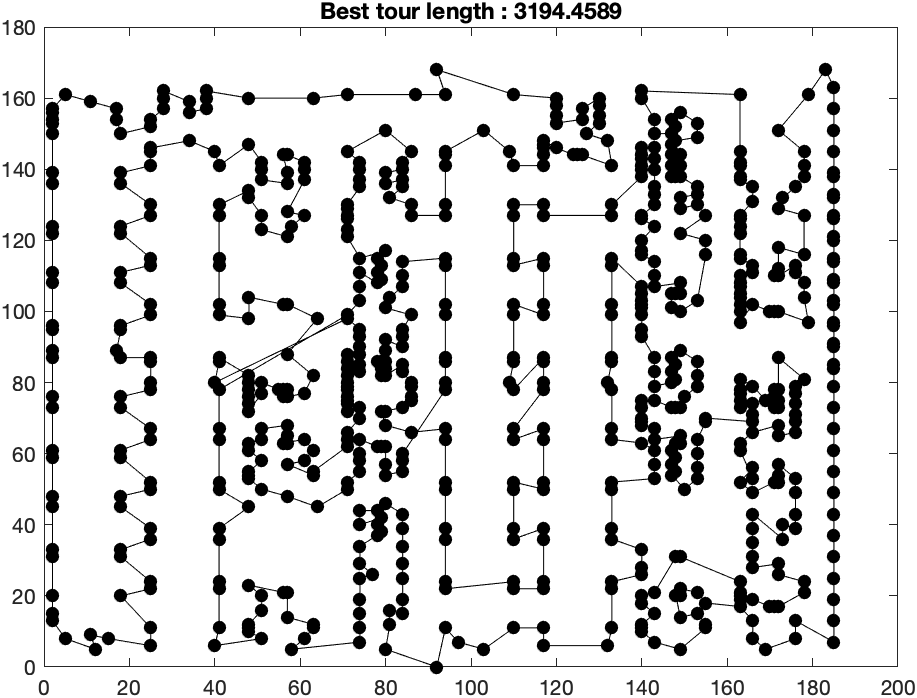
\includegraphics[width=\textwidth]{benchmarks/rbx711.png}
		\caption{\texttt{rbx711}}
    	\end{subfigure}
\caption*{Results on benchmarks. Error rates of 1.72\%, 4.33\%, 4.7\% and 2.55\% respectively.}
\label{fig:bench1}
\end{figure}

\begin{table}[h]
\centering
\footnotesize
\begin{tabular}{c|c|c|c|c|c|c}
\textit{Crossover} & \textit{Mutation} & \textit{Population Size} & \textit{Crossover Rate (\%)} & \textit{Mutation Rate (\%)} & \textit{Elitism (\%)} & \textit{Generations} \\\hline 
Unnamed & Simple Inversion & 300 & 50\% & 40\% & 5\% & 1000
\end{tabular}
\caption{Parameters used for the tests on the benchmarks. No stopping criterion was used.}
\label{tab:bench1}
\end{table}

\fakesection{Other Tasks}{}

Until now, most of the analysis was done with the purpose of finding a good solution for every benchmark. Other facets that were neglected to some extent are selective pressure and diversity. Those can be crucial to prevent premature convergence and increase the probability of finding the better - or even the optimal - solution(s). Therefor, some attention was given to strategies like tournament selection.

\fakesubsection{Parent Selection}{\hfill\small\texttt{/selection/*.m}}

The most interesting parent selection strategy that was implemented is probably tournament selection. Both tournament selection with - and without replacement were implemented. Results of some basic experiments are displayed in tabel \ref{tab:parentres}.\\

\par\noindent While the rank-based method may appear preferable, in all runs where it was used the algorithm stopped early on because the stopping criterion was met (no improvement was seen for 100 generations in a row). Whereas when tournament selection with replacement ($k=2$) was used this was not the case.

\begin{table}[h]
\centering
\footnotesize
\begin{tabular}{c|c|c|c|c|c|c}
\textit{Crossover} & \textit{Mutation} & \textit{Population Size} & \textit{Crossover Rate} & \textit{Mutation Rate} & \textit{Elitism} & \textit{Generations} \\\hline 
\texttt{OX1} & Reciprocal Exchange & 300 & 50\% & 40\% & 5\% & 1000
\end{tabular}
\caption{Parameters used for tests on various types of parent selection. A stopping criterion was used.}
\label{tab:parent}
\end{table}

\begin{table}[h]
\centering
\footnotesize
\begin{tabular}{c|c|c|c|c|c}
\textit{FPS} & \textit{Linear Rank} & \textit{TNM ($k=2$)} & \textit{TNM ($k=10$)} & \textit{TNM ($k=20$)} & \textit{TNMWR $k=2$ (no replacement)}  \\\hline 
49.23/126.00 & 41.35/51.58 & 41.31/75.47 & 42.15/47.58 & 42.66/47.85 & 42.86/87.21
\\
1045.12/2654.36 & 723.89/867.44 & 773.79/1358.97 & 793.34/867.53 & 811.02/878.55 & 767.45/1531.66
\end{tabular}
\caption{Results of experiments with several parent selection strategies. \textit{TNM} = Tournament selection. \textit{TNMWR} = Tournament selection without replacement Average of best and average fitness across 30 runs is displayed. First row represents experiments on a tour of 25 cities, second row are experiments on the belgian tour (41 cities). The results are equivalent for both tours.}
\label{tab:parentres}
\end{table}

\noindent To elaborate on this : what's not shown is the number of generations it took for the stopping criterion to be met. In the case of the (linear) rank-based selection it was met in all runs, often fairly early on (within 400 generations). In the case of fitness-proportionate selection it was frequently met (especially in the shorter tour of 25 cities). And in the case of tournament selection it depended on the value of $k$ and whether or not replacement was used. For $k=10$ it was met within 300 generations in most cases, for $k=20$ within 200 generations. Clearly, the value of $k$ influences selective pressure and setting it too high may lead to premature convergence. When tournament selection without replacement was used, the number of generations before the stopping criterion was met increased sharply (sometimes it wasn't even met within 1000 generations). This is not surprising since lesser individuals get a higher chance of surviving (as noted in Eiben's book).\\

\par\noindent Non-linear ranking turned out to be fairly useful as well, but tournament selection looked most likeable as a strategy as it can be run in parallel and its arguments allow one to control selective pressure quite easily (higher $k$ values clearly increased the average fitness value which is an - admittedly somewhat poor - metric for diversity).

\fakesubsection{Survivor Selection}{\hfill\small\texttt{/reinsertion/*.m}}

Out of the three survivor selection strategies that were implemented - $\mu+\lambda$, round robin and uniform selection - the first two led to premature convergence and the latter was highly unpredictable and definitely not particularly useful. Any of the parent selection methods can be used for survivor selection as well. Round-robin and $\mu+\lambda$ consider the merged offspring - and parent population. If diversity is not preserved in some way they select parents more and more often (because as the algorithm converges these tend to have higher fitness values). When the crossover - and mutation rate are high it it less of a problem.

\fakesubsection{Diversity Preservation}{}

An island model was implemented in which the population is divided into islands if it is large enough. Every island hosts at least 25 individuals and the best ones are transferred from one to the other every so often (leading to periodic drops in average and worst fitness values throughout the generations). It obviously helped with diversity but not in the way tournament selection does ; if there was premature convergence in some algorithm, using the island model tends to transfer that problem to most of the islands themselves (as in, most islands experience a similar degree of convergence). \textit{After} migration the degree of convergence drops (this is based on visual analysis of the graphs in the GUI). \\

\par\noindent One way to measure diversity is by counting the number of unique fitness values in the population (admittedly not a perfect measure since different genotypes may have the same fitness value). The median number of uniques across generations typically turned out to be higher when using the island model. Even the mean was nearly higher despite the fact that during migration the worst individuals in islands are replaced by the best individuals in other islands, which leads to a stark but short-lived drop in the number of unique fitness values, followed by an increase (until it reaches a value that's typically higher than what it was before migration). For example, the average of the median of the number of unique fitness values across 250 generations (for 30 runs on the belgian tour) was calculated to be 75 and 63 (with and without island model).

%\begin{figure}[H]
%\centering
%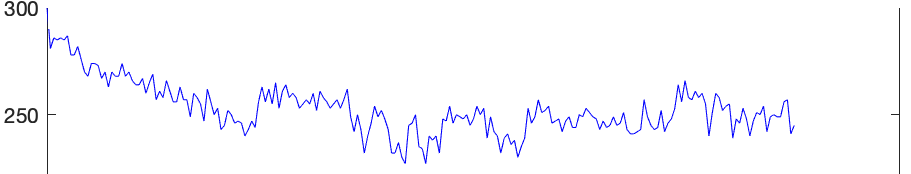
\includegraphics[width=0.8\textwidth]{island/a.png}
%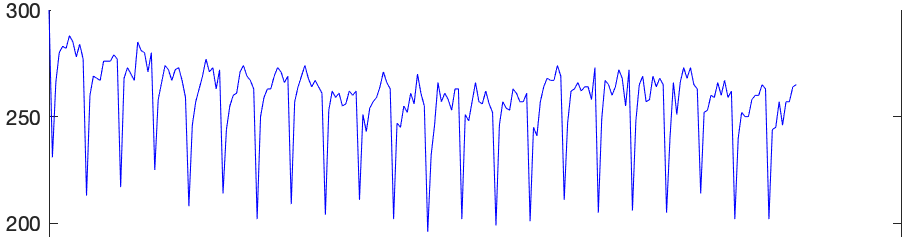
\includegraphics[width=0.8\textwidth]{island/b.png}
%\end{figure}

\fakesubsection{Adaptive Parameter Tuning}{}

It would seem that, as several good solutions have been found after quite a few generations, increased frequency of mutation and reduced frequency of local optimisation (if hybridisation is activated) would prove useful by allowing for a more liberal exploration of the search space. Therefor, an adaptive parameter strategy was implemented which does just that. Instead of seeing interesting new solutions emerge, the average fitness just kept on diverging. Probably because the search became equivalent to a rather random search.

\fakesubsection{Further Hybridisation}{\hfill\small\texttt{/hybridisation/nearest\_neighbor.m}}

Seeding is a frequently used technique to give a head start. There's several possible approximate solutions for the TSP that can be used for this purpose. One of them is a nearest neighbour solution where a random city is picked and a tour is formed by repeatedly selecting the city nearest to the current one until all of them have been selected. This works well until at the end the remaining edges have to be added, often at high cost. It provides a decent initial solution which is retained through elitism and may provide inspiration for subsequent tours (or lead the algorithm towards a local optimum). In most experiments the resulting initial tour turned out to have a length that's within 15\% of the optimal one, and the genetic algorithm caused further improvements until (in a typical run) the resulting tour ended up within about 6\% of the optimum. No \textit{kd}-tree was used as a seed is only constructed once for every run which (in comparison to a whole run) takes little time. Unsurprisingly, however, it barely helped with finding a \textit{truly} good tour. Instead it improved the average best tour found across runs.

\fakesection{Benchmarks with Heuristics}{}

A final test on the benchmarks was done, this time with \textit{2-opt} enabled. It was not applied in each generation, only every so often because it is still a fairly costly operation (as the number of generations increases it is applied less and less to increase the chances of getting out of a local minimum). Tournament selection and the island model was enabled.

\begin{table}[h]
\centering
\footnotesize
\begin{tabular}{c|c|c|c|c|c|c}
\textit{Crossover} & \textit{Mutation} & \textit{Population Size} & \textit{Crossover Rate (\%)} & \textit{Mutation Rate (\%)} & \textit{Elitism (\%)} & \textit{Generations} \\\hline 
Unnamed & Reciprocal Exchange & 300 & 50\% & 40\% & 5\% & 1000
\end{tabular}
\caption{Parameters used for the final tests on the benchmarks. No stopping criterion was used.}
\label{tab:par2}
\end{table}

\begin{figure}[H]
	\centering
%
	\begin{subfigure}[b]{0.45\textwidth}
		\centering
		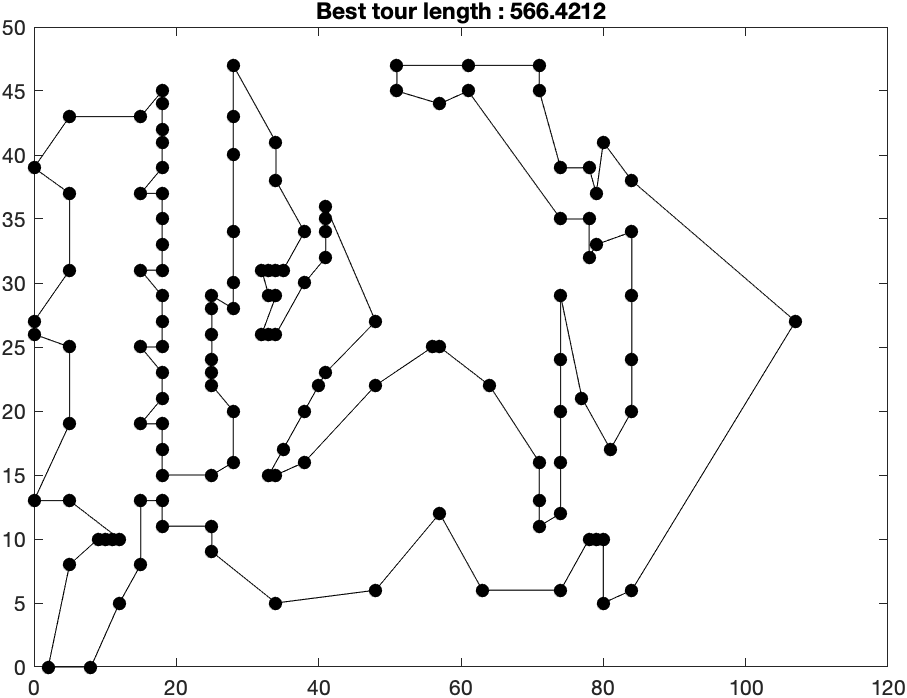
\includegraphics[width=\textwidth]{benchmarks/final/xqf131.png}
		\caption{\texttt{xqf131}}
    	\end{subfigure}
	\begin{subfigure}[b]{0.45\textwidth}
		\centering
		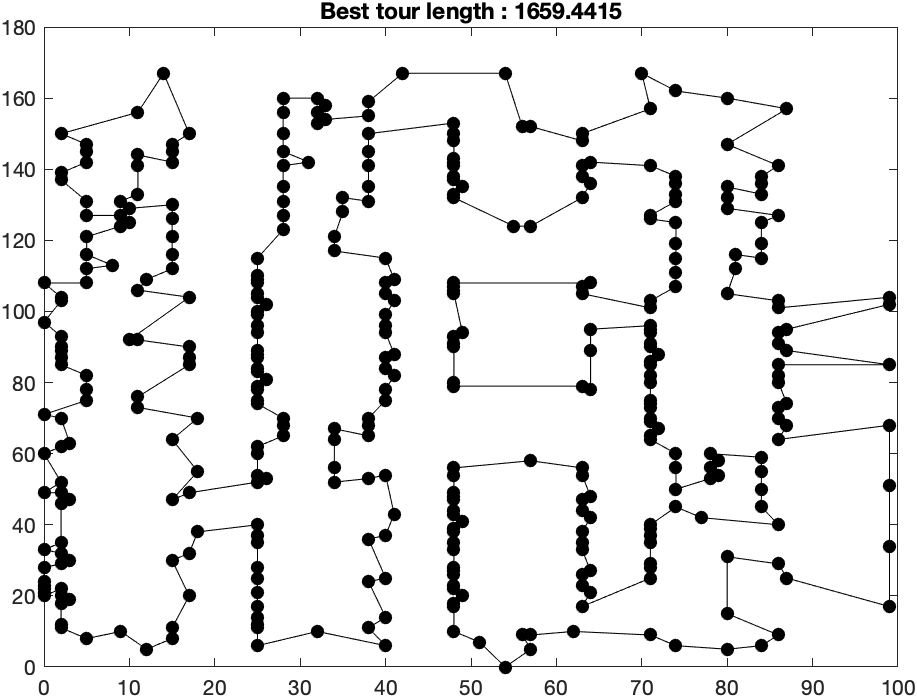
\includegraphics[width=\textwidth]{benchmarks/final/bcl380.png}
		\caption{\texttt{bcl380}}
    	\end{subfigure}
	\begin{subfigure}[b]{0.45\textwidth}
		\centering
		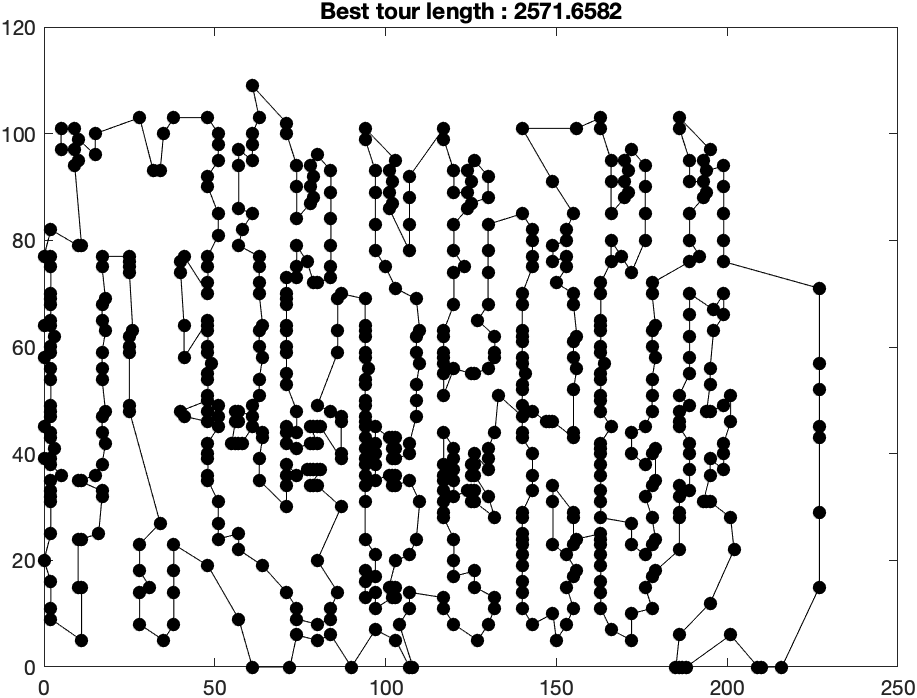
\includegraphics[width=\textwidth]{benchmarks/final/xql662.png}
		\caption{\texttt{xql662}}
    	\end{subfigure}
	\begin{subfigure}[b]{0.45\textwidth}
		\centering
		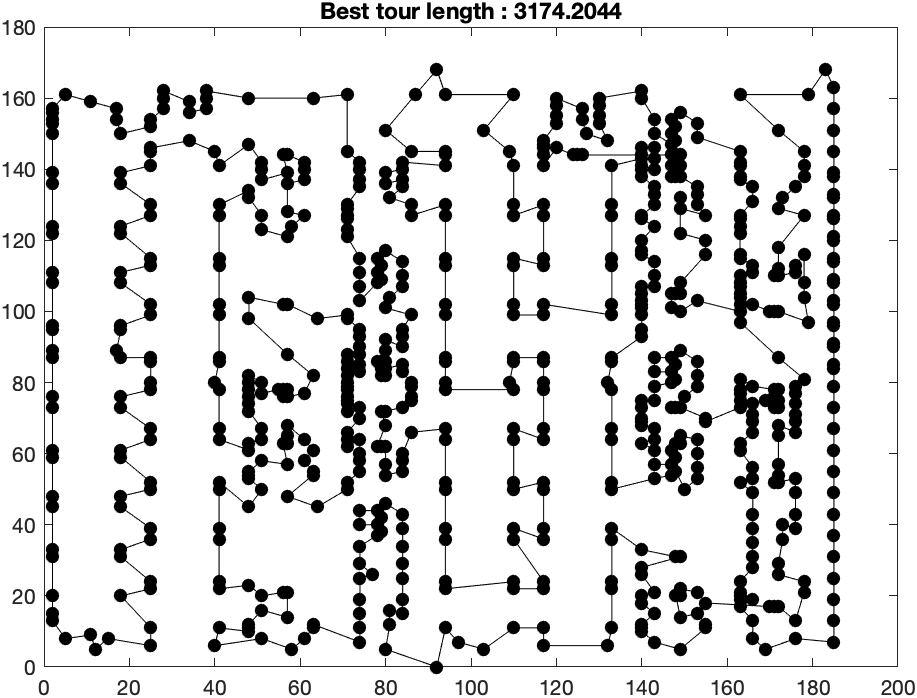
\includegraphics[width=\textwidth]{benchmarks/final/rbx711.png}
		\caption{\texttt{rbx711}}
    	\end{subfigure}
\caption{Results on benchmarks, this time \textit{with} heuristics like \textit{2-opt}. Error rates of 0.43\%, 2.37\%, 2.33\% and 1.9\% respectively.}
\label{fig:bench1}
\end{figure}

\newpage
\advance\voffset by -0.6cm
%\newgeometry{top=7mm, bottom=7mm}

%%%%%%%%%%%%%%%%%%%%%%%%%%%%%%%%%%%%%%%%%%%%%%%%%%%%%%%%%%%%%%%%%%%%%%%%%%%%%%%%%%%%%%%%%%%%%%%%%%%%%%%%%
%%%%%%%%%%%%%%%%%%%%%%%%%%%%%%%%%%%%%%%%%%%%%%%%%%%%%%%%%%%%%%%%%%%%%%%%%%%%%%%%%%%%%%%%%%%%%%%%%%%%%%%%%
%%%%%%%%%%%%%%%%%%%%%%%%%%%%%%%%%%%%%%%%%%%%%%%%%%%%%%%%%%%%%%%%%%%%%%%%%%%%%%%%%%%%%%%%%%%%%%%%%%%%%%%%%

\pagenumbering{gobble}
\begin{table}[H]
\centering
\footnotesize
{\renewcommand{\arraystretch}{1}}
\begin{tabular}{ccc|c|c|c|c|c}
\textit{Crossover Rate} & \textit{Mutation Rate} & \textit{Elitism} & \texttt{rondrit025} & \texttt{rondrit070} & \texttt{rondrit0127} & \texttt{belgiumtour} & \textit{Total Time (s)} \\\hline
5 & 10 & 1 & \cellcolor{gray!80}39.88 & \cellcolor{gray!13}1129.53 & \cellcolor{gray!1}301.73 & \cellcolor{gray!67}705.33 & 3.16\\
5 & 10 & 5 & \cellcolor{gray!80}39.85 & \cellcolor{gray!16}1111.11 & \cellcolor{gray!1}295.07 & \cellcolor{gray!67}704.37 & 2.92\\
5 & 10 & 10 & \cellcolor{gray!80}39.88 & \cellcolor{gray!13}1128.86 & \cellcolor{gray!1}292.94 & \cellcolor{gray!64}714.93 & 3.07\\
25 & 10 & 1 & \cellcolor{gray!80}39.85 & \cellcolor{gray!20}1089.23 & \cellcolor{gray!1}277.36 & \cellcolor{gray!63}717.66 & 6.33\\
25 & 10 & 5 & \cellcolor{gray!79}39.95 & \cellcolor{gray!22}1078.36 & \cellcolor{gray!1}271.84 & \cellcolor{gray!68}701.80 & 5.30\\
25 & 10 & 10 & \cellcolor{gray!80}39.81 & \cellcolor{gray!25}1060.66 & \cellcolor{gray!1}269.12 & \cellcolor{gray!68}701.97 & 5.54\\
50 & 10 & 1 & \cellcolor{gray!80}39.81 & \cellcolor{gray!1}1252.28 & \cellcolor{gray!1}333.35 & \cellcolor{gray!58}733.01 & 10.01\\
50 & 10 & 5 & \cellcolor{gray!80}39.81 & \cellcolor{gray!27}1047.86 & \cellcolor{gray!1}272.19 & \cellcolor{gray!68}701.33 & 9.16\\
50 & 10 & 10 & \cellcolor{gray!80}39.81 & \cellcolor{gray!26}1052.85 & \cellcolor{gray!1}267.24 & \cellcolor{gray!71}689.64 & 8.89\\
75 & 10 & 1 & \cellcolor{gray!1}50.24 & \cellcolor{gray!1}2044.69 & \cellcolor{gray!1}443.77 & \cellcolor{gray!1}1285.26 & 15.39\\
75 & 10 & 5 & \cellcolor{gray!80}39.81 & \cellcolor{gray!1}1398.13 & \cellcolor{gray!1}325.15 & \cellcolor{gray!42}784.33 & 15.31\\
75 & 10 & 10 & \cellcolor{gray!80}39.81 & \cellcolor{gray!11}1139.36 & \cellcolor{gray!1}291.46 & \cellcolor{gray!68}701.02 & 13.24\\
95 & 10 & 1 & \cellcolor{gray!1}57.56 & \cellcolor{gray!1}2332.09 & \cellcolor{gray!1}462.01 & \cellcolor{gray!1}1465.70 & 18.95\\
95 & 10 & 5 & \cellcolor{gray!24}45.43 & \cellcolor{gray!1}1888.66 & \cellcolor{gray!1}398.31 & \cellcolor{gray!1}1198.29 & 17.31\\
95 & 10 & 10 & \cellcolor{gray!80}39.81 & \cellcolor{gray!1}1444.34 & \cellcolor{gray!1}354.56 & \cellcolor{gray!40}790.83 & 16.69\\
5 & 25 & 1 & \cellcolor{gray!80}39.85 & \cellcolor{gray!37}984.46 & \cellcolor{gray!1}275.61 & \cellcolor{gray!73}684.16 & 3.79\\
5 & 25 & 5 & \cellcolor{gray!80}39.81 & \cellcolor{gray!38}982.26 & \cellcolor{gray!1}262.45 & \cellcolor{gray!73}685.49 & 3.48\\
5 & 25 & 10 & \cellcolor{gray!80}39.81 & \cellcolor{gray!45}939.78 & \cellcolor{gray!3}259.67 & \cellcolor{gray!75}677.71 & 3.46\\
25 & 25 & 1 & \cellcolor{gray!80}39.81 & \cellcolor{gray!17}1107.00 & \cellcolor{gray!1}274.10 & \cellcolor{gray!71}691.25 & 7.05\\
25 & 25 & 5 & \cellcolor{gray!80}39.81 & \cellcolor{gray!34}1005.26 & \cellcolor{gray!2}260.25 & \cellcolor{gray!71}690.62 & 6.43\\
25 & 25 & 10 & \cellcolor{gray!80}39.88 & \cellcolor{gray!31}1023.40 & \cellcolor{gray!22}239.45 & \cellcolor{gray!75}678.65 & 5.99\\
50 & 25 & 1 & \cellcolor{gray!79}39.95 & \cellcolor{gray!1}1474.90 & \cellcolor{gray!1}333.94 & \cellcolor{gray!12}883.15 & 11.77\\
50 & 25 & 5 & \cellcolor{gray!80}39.85 & \cellcolor{gray!20}1089.82 & \cellcolor{gray!1}282.48 & \cellcolor{gray!74}680.63 & 10.57\\
50 & 25 & 10 & \cellcolor{gray!80}39.81 & \cellcolor{gray!36}992.49 & \cellcolor{gray!1}270.82 & \cellcolor{gray!75}677.26 & 9.88\\
75 & 25 & 1 & \cellcolor{gray!1}53.05 & \cellcolor{gray!1}2013.87 & \cellcolor{gray!1}422.98 & \cellcolor{gray!1}1273.33 & 16.31\\
75 & 25 & 5 & \cellcolor{gray!76}40.26 & \cellcolor{gray!1}1388.90 & \cellcolor{gray!1}328.45 & \cellcolor{gray!12}881.81 & 15.09\\
75 & 25 & 10 & \cellcolor{gray!80}39.81 & \cellcolor{gray!2}1196.01 & \cellcolor{gray!1}296.75 & \cellcolor{gray!73}684.32 & 13.83\\
95 & 25 & 1 & \cellcolor{gray!1}58.29 & \cellcolor{gray!1}2324.97 & \cellcolor{gray!1}469.66 & \cellcolor{gray!1}1495.37 & 20.09\\
95 & 25 & 5 & \cellcolor{gray!43}43.54 & \cellcolor{gray!1}1733.56 & \cellcolor{gray!1}400.03 & \cellcolor{gray!1}1129.13 & 18.53\\
95 & 25 & 10 & \cellcolor{gray!80}39.81 & \cellcolor{gray!1}1458.97 & \cellcolor{gray!1}350.66 & \cellcolor{gray!46}772.29 & 17.59\\
5 & 50 & 1 & \cellcolor{gray!80}39.81 & \cellcolor{gray!28}1037.46 & \cellcolor{gray!1}263.77 & \cellcolor{gray!66}706.61 & 4.92\\
5 & 50 & 5 & \cellcolor{gray!80}39.81 & \cellcolor{gray!44}941.95 & \cellcolor{gray!13}249.01 & \cellcolor{gray!75}677.22 & 4.48\\
5 & 50 & 10 & \cellcolor{gray!80}39.85 & \cellcolor{gray!42}957.15 & \cellcolor{gray!15}246.60 & \cellcolor{gray!71}690.40 & 4.75\\
25 & 50 & 1 & \cellcolor{gray!80}39.81 & \cellcolor{gray!13}1129.27 & \cellcolor{gray!1}287.48 & \cellcolor{gray!39}794.02 & 8.40\\
25 & 50 & 5 & \cellcolor{gray!80}39.81 & \cellcolor{gray!34}1004.02 & \cellcolor{gray!6}255.89 & \cellcolor{gray!73}684.30 & 7.99\\
25 & 50 & 10 & \cellcolor{gray!80}39.85 & \cellcolor{gray!37}989.45 & \cellcolor{gray!10}252.58 & \cellcolor{gray!74}681.72 & 7.07\\
50 & 50 & 1 & \cellcolor{gray!56}42.25 & \cellcolor{gray!1}1518.22 & \cellcolor{gray!1}342.51 & \cellcolor{gray!2}916.12 & 12.75\\
50 & 50 & 5 & \cellcolor{gray!80}39.81 & \cellcolor{gray!8}1162.22 & \cellcolor{gray!1}278.63 & \cellcolor{gray!71}691.92 & 11.67\\
50 & 50 & 10 & \cellcolor{gray!80}39.81 & \cellcolor{gray!25}1056.73 & \cellcolor{gray!1}270.87 & \cellcolor{gray!72}687.67 & 10.79\\
75 & 50 & 1 & \cellcolor{gray!19}45.89 & \cellcolor{gray!1}2040.46 & \cellcolor{gray!1}417.27 & \cellcolor{gray!1}1160.69 & 17.57\\
75 & 50 & 5 & \cellcolor{gray!76}40.23 & \cellcolor{gray!1}1381.74 & \cellcolor{gray!1}323.16 & \cellcolor{gray!28}830.28 & 16.54\\
75 & 50 & 10 & \cellcolor{gray!80}39.81 & \cellcolor{gray!1}1274.47 & \cellcolor{gray!1}306.12 & \cellcolor{gray!54}746.85 & 15.28\\
95 & 50 & 1 & \cellcolor{gray!1}56.11 & \cellcolor{gray!1}2190.59 & \cellcolor{gray!1}463.83 & \cellcolor{gray!1}1393.32 & 20.43\\
95 & 50 & 5 & \cellcolor{gray!41}43.70 & \cellcolor{gray!1}1730.25 & \cellcolor{gray!1}387.40 & \cellcolor{gray!1}1015.05 & 19.47\\
95 & 50 & 10 & \cellcolor{gray!78}40.05 & \cellcolor{gray!1}1516.67 & \cellcolor{gray!1}339.17 & \cellcolor{gray!9}892.06 & 18.64\\
5 & 75 & 1 & \cellcolor{gray!80}39.81 & \cellcolor{gray!7}1163.46 & \cellcolor{gray!1}269.17 & \cellcolor{gray!34}812.60 & 6.57\\
5 & 75 & 5 & \cellcolor{gray!80}39.81 & \cellcolor{gray!44}945.76 & \cellcolor{gray!22}238.76 & \cellcolor{gray!68}700.27 & 6.26\\
5 & 75 & 10 & \cellcolor{gray!80}39.85 & \cellcolor{gray!46}930.06 & \cellcolor{gray!21}240.42 & \cellcolor{gray!74}682.05 & 6.05\\
25 & 75 & 1 & \cellcolor{gray!76}40.26 & \cellcolor{gray!1}1276.73 & \cellcolor{gray!1}287.03 & \cellcolor{gray!19}859.56 & 10.01\\
25 & 75 & 5 & \cellcolor{gray!80}39.81 & \cellcolor{gray!33}1008.69 & \cellcolor{gray!13}248.93 & \cellcolor{gray!64}714.51 & 9.28\\
25 & 75 & 10 & \cellcolor{gray!80}39.85 & \cellcolor{gray!34}1003.08 & \cellcolor{gray!18}243.49 & \cellcolor{gray!64}713.66 & 8.09\\
50 & 75 & 1 & \cellcolor{gray!62}41.63 & \cellcolor{gray!1}1520.14 & \cellcolor{gray!1}338.83 & \cellcolor{gray!1}929.25 & 13.45\\
50 & 75 & 5 & \cellcolor{gray!80}39.81 & \cellcolor{gray!12}1136.45 & \cellcolor{gray!1}279.42 & \cellcolor{gray!56}740.43 & 12.74\\
50 & 75 & 10 & \cellcolor{gray!80}39.81 & \cellcolor{gray!23}1071.56 & \cellcolor{gray!1}281.17 & \cellcolor{gray!71}689.91 & 12.13\\
75 & 75 & 1 & \cellcolor{gray!5}47.22 & \cellcolor{gray!1}1958.61 & \cellcolor{gray!1}406.44 & \cellcolor{gray!1}1221.32 & 17.49\\
75 & 75 & 5 & \cellcolor{gray!78}40.04 & \cellcolor{gray!1}1388.59 & \cellcolor{gray!1}312.78 & \cellcolor{gray!19}860.72 & 17.59\\
75 & 75 & 10 & \cellcolor{gray!80}39.85 & \cellcolor{gray!1}1292.43 & \cellcolor{gray!1}308.98 & \cellcolor{gray!43}780.71 & 18.28\\
95 & 75 & 1 & \cellcolor{gray!1}59.41 & \cellcolor{gray!1}2290.11 & \cellcolor{gray!1}469.52 & \cellcolor{gray!1}1480.32 & 23.01\\
95 & 75 & 5 & \cellcolor{gray!66}41.28 & \cellcolor{gray!1}1760.24 & \cellcolor{gray!1}384.56 & \cellcolor{gray!1}1146.44 & 21.89\\
95 & 75 & 10 & \cellcolor{gray!72}40.63 & \cellcolor{gray!1}1539.35 & \cellcolor{gray!1}352.51 & \cellcolor{gray!1}930.64 & 19.27\\
5 & 95 & 1 & \cellcolor{gray!75}40.35 & \cellcolor{gray!1}1215.18 & \cellcolor{gray!1}263.81 & \cellcolor{gray!31}821.78 & 7.13\\
5 & 95 & 5 & \cellcolor{gray!80}39.85 & \cellcolor{gray!31}1021.89 & \cellcolor{gray!17}244.37 & \cellcolor{gray!65}709.13 & 6.58\\
5 & 95 & 10 & \cellcolor{gray!80}39.81 & \cellcolor{gray!33}1009.70 & \cellcolor{gray!25}236.50 & \cellcolor{gray!69}695.87 & 6.51\\
25 & 95 & 1 & \cellcolor{gray!56}42.21 & \cellcolor{gray!1}1354.51 & \cellcolor{gray!1}297.81 & \cellcolor{gray!13}878.39 & 10.48\\
25 & 95 & 5 & \cellcolor{gray!80}39.88 & \cellcolor{gray!21}1082.92 & \cellcolor{gray!1}262.25 & \cellcolor{gray!62}719.63 & 10.23\\
25 & 95 & 10 & \cellcolor{gray!80}39.81 & \cellcolor{gray!25}1060.29 & \cellcolor{gray!1}263.16 & \cellcolor{gray!67}703.41 & 9.34\\
50 & 95 & 1 & \cellcolor{gray!16}46.21 & \cellcolor{gray!1}1435.87 & \cellcolor{gray!1}339.08 & \cellcolor{gray!1}985.20 & 15.25\\
50 & 95 & 5 & \cellcolor{gray!80}39.81 & \cellcolor{gray!2}1198.67 & \cellcolor{gray!1}290.15 & \cellcolor{gray!30}823.71 & 13.31\\
50 & 95 & 10 & \cellcolor{gray!80}39.88 & \cellcolor{gray!9}1152.10 & \cellcolor{gray!1}274.71 & \cellcolor{gray!48}766.47 & 12.85\\
75 & 95 & 1 & \cellcolor{gray!1}47.77 & \cellcolor{gray!1}1908.15 & \cellcolor{gray!1}404.15 & \cellcolor{gray!1}1178.48 & 20.32\\
75 & 95 & 5 & \cellcolor{gray!74}40.49 & \cellcolor{gray!1}1384.93 & \cellcolor{gray!1}336.02 & \cellcolor{gray!3}913.31 & 18.70\\
75 & 95 & 10 & \cellcolor{gray!74}40.49 & \cellcolor{gray!1}1398.93 & \cellcolor{gray!1}316.32 & \cellcolor{gray!33}814.54 & 17.73\\
95 & 95 & 1 & \cellcolor{gray!1}57.91 & \cellcolor{gray!1}2228.48 & \cellcolor{gray!1}460.84 & \cellcolor{gray!1}1418.74 & 21.39\\
95 & 95 & 5 & \cellcolor{gray!49}42.92 & \cellcolor{gray!1}1731.17 & \cellcolor{gray!1}390.41 & \cellcolor{gray!1}1120.34 & 21.23\\
95 & 95 & 10 & \cellcolor{gray!68}41.07 & \cellcolor{gray!1}1649.37 & \cellcolor{gray!1}362.66 & \cellcolor{gray!1}1025.49 & 19.49
\end{tabular}
\caption{Results of 75 configurations (population size of 150). The grayscale values of the cells are calibrated against the minimum and maximum for all tests (from table \ref{tab:res1} to \ref{tab:res5}). Darker cells represent better solutions. No stopping criterion was used, maximum number of generations was set to 250. Each configuration was run 10 times.}
\label{tab:res1}
\end{table}

%%%%%%%%%%%%%%%%%%%%%%%%%%%%%%%%%%%%%%%%%%%%%%%%%%%%%%%%%%%%%%%%%%%%%%%%%%%%%%%%%%%%%%%%%%%%%%%%%%%%%%%%%
%%%%%%%%%%%%%%%%%%%%%%%%%%%%%%%%%%%%%%%%%%%%%%%%%%%%%%%%%%%%%%%%%%%%%%%%%%%%%%%%%%%%%%%%%%%%%%%%%%%%%%%%%
%%%%%%%%%%%%%%%%%%%%%%%%%%%%%%%%%%%%%%%%%%%%%%%%%%%%%%%%%%%%%%%%%%%%%%%%%%%%%%%%%%%%%%%%%%%%%%%%%%%%%%%%%

\pagenumbering{gobble}
\begin{table}[H]
\centering

\footnotesize
{\renewcommand{\arraystretch}{1}}
\begin{tabular}{ccc|c|c|c|c|c}
\textit{Crossover Rate} & \textit{Mutation Rate} & \textit{Elitism} & \texttt{rondrit025} & \texttt{rondrit070} & \texttt{rondrit0127} & \texttt{belgiumtour} & \textit{Total Time (s)} \\\hline
5 & 10 & 1 & \cellcolor{gray!80}39.81 & \cellcolor{gray!30}1026.32 & \cellcolor{gray!1}277.45 & \cellcolor{gray!71}689.66 & 5.42\\
5 & 10 & 5 & \cellcolor{gray!80}39.85 & \cellcolor{gray!36}995.24 & \cellcolor{gray!1}267.05 & \cellcolor{gray!73}684.67 & 4.70\\
5 & 10 & 10 & \cellcolor{gray!80}39.85 & \cellcolor{gray!29}1034.40 & \cellcolor{gray!1}271.66 & \cellcolor{gray!75}677.14 & 4.97\\
25 & 10 & 1 & \cellcolor{gray!80}39.81 & \cellcolor{gray!40}967.10 & \cellcolor{gray!1}267.26 & \cellcolor{gray!74}680.93 & 12.03\\
25 & 10 & 5 & \cellcolor{gray!80}39.85 & \cellcolor{gray!44}942.67 & \cellcolor{gray!13}248.75 & \cellcolor{gray!75}679.28 & 11.62\\
25 & 10 & 10 & \cellcolor{gray!80}39.81 & \cellcolor{gray!44}942.36 & \cellcolor{gray!10}252.09 & \cellcolor{gray!74}679.51 & 10.81\\
50 & 10 & 1 & \cellcolor{gray!80}39.85 & \cellcolor{gray!4}1181.41 & \cellcolor{gray!1}308.58 & \cellcolor{gray!68}699.21 & 20.95\\
50 & 10 & 5 & \cellcolor{gray!80}39.85 & \cellcolor{gray!36}995.10 & \cellcolor{gray!3}260.14 & \cellcolor{gray!75}677.24 & 19.37\\
50 & 10 & 10 & \cellcolor{gray!80}39.85 & \cellcolor{gray!46}932.83 & \cellcolor{gray!11}251.33 & \cellcolor{gray!74}681.64 & 17.94\\
75 & 10 & 1 & \cellcolor{gray!1}49.77 & \cellcolor{gray!1}1909.07 & \cellcolor{gray!1}413.22 & \cellcolor{gray!1}1189.79 & 34.17\\
75 & 10 & 5 & \cellcolor{gray!80}39.81 & \cellcolor{gray!1}1331.43 & \cellcolor{gray!1}312.04 & \cellcolor{gray!48}764.27 & 28.72\\
75 & 10 & 10 & \cellcolor{gray!80}39.81 & \cellcolor{gray!16}1110.10 & \cellcolor{gray!1}301.25 & \cellcolor{gray!75}679.07 & 25.53\\
95 & 10 & 1 & \cellcolor{gray!1}52.69 & \cellcolor{gray!1}2099.32 & \cellcolor{gray!1}436.22 & \cellcolor{gray!1}1388.94 & 41.01\\
95 & 10 & 5 & \cellcolor{gray!47}43.11 & \cellcolor{gray!1}1699.08 & \cellcolor{gray!1}384.74 & \cellcolor{gray!1}1015.50 & 37.93\\
95 & 10 & 10 & \cellcolor{gray!80}39.81 & \cellcolor{gray!1}1435.37 & \cellcolor{gray!1}347.33 & \cellcolor{gray!29}826.52 & 36.89\\
5 & 25 & 1 & \cellcolor{gray!80}39.81 & \cellcolor{gray!48}921.40 & \cellcolor{gray!7}255.56 & \cellcolor{gray!80}660.77 & 8.42\\
5 & 25 & 5 & \cellcolor{gray!80}39.81 & \cellcolor{gray!56}871.97 & \cellcolor{gray!6}255.94 & \cellcolor{gray!74}681.10 & 7.11\\
5 & 25 & 10 & \cellcolor{gray!80}39.81 & \cellcolor{gray!49}915.70 & \cellcolor{gray!10}252.50 & \cellcolor{gray!75}677.05 & 6.94\\
25 & 25 & 1 & \cellcolor{gray!80}39.81 & \cellcolor{gray!31}1021.10 & \cellcolor{gray!1}263.19 & \cellcolor{gray!75}677.28 & 12.73\\
25 & 25 & 5 & \cellcolor{gray!80}39.81 & \cellcolor{gray!48}923.51 & \cellcolor{gray!17}244.58 & \cellcolor{gray!77}672.53 & 12.60\\
25 & 25 & 10 & \cellcolor{gray!80}39.85 & \cellcolor{gray!51}904.66 & \cellcolor{gray!24}237.40 & \cellcolor{gray!79}664.40 & 12.21\\
50 & 25 & 1 & \cellcolor{gray!80}39.81 & \cellcolor{gray!1}1303.49 & \cellcolor{gray!1}317.24 & \cellcolor{gray!48}765.23 & 21.33\\
50 & 25 & 5 & \cellcolor{gray!80}39.81 & \cellcolor{gray!34}1002.86 & \cellcolor{gray!1}267.11 & \cellcolor{gray!78}666.79 & 19.68\\
50 & 25 & 10 & \cellcolor{gray!80}39.81 & \cellcolor{gray!36}990.84 & \cellcolor{gray!8}254.46 & \cellcolor{gray!74}680.47 & 18.79\\
75 & 25 & 1 & \cellcolor{gray!36}44.17 & \cellcolor{gray!1}1799.59 & \cellcolor{gray!1}397.71 & \cellcolor{gray!1}1053.97 & 32.16\\
75 & 25 & 5 & \cellcolor{gray!80}39.81 & \cellcolor{gray!1}1263.23 & \cellcolor{gray!1}303.54 & \cellcolor{gray!40}792.28 & 30.09\\
75 & 25 & 10 & \cellcolor{gray!80}39.81 & \cellcolor{gray!13}1127.83 & \cellcolor{gray!1}288.70 & \cellcolor{gray!69}697.76 & 29.91\\
95 & 25 & 1 & \cellcolor{gray!1}52.78 & \cellcolor{gray!1}2121.78 & \cellcolor{gray!1}449.08 & \cellcolor{gray!1}1309.36 & 39.69\\
95 & 25 & 5 & \cellcolor{gray!62}41.60 & \cellcolor{gray!1}1663.95 & \cellcolor{gray!1}376.11 & \cellcolor{gray!1}993.88 & 40.59\\
95 & 25 & 10 & \cellcolor{gray!80}39.81 & \cellcolor{gray!1}1476.09 & \cellcolor{gray!1}325.93 & \cellcolor{gray!24}842.27 & 36.03\\
5 & 50 & 1 & \cellcolor{gray!80}39.81 & \cellcolor{gray!42}956.59 & \cellcolor{gray!23}238.68 & \cellcolor{gray!75}677.69 & 10.07\\
5 & 50 & 5 & \cellcolor{gray!80}39.81 & \cellcolor{gray!52}898.48 & \cellcolor{gray!22}239.26 & \cellcolor{gray!79}665.35 & 10.19\\
5 & 50 & 10 & \cellcolor{gray!80}39.81 & \cellcolor{gray!58}858.82 & \cellcolor{gray!33}227.84 & \cellcolor{gray!75}678.52 & 8.44\\
25 & 50 & 1 & \cellcolor{gray!80}39.81 & \cellcolor{gray!24}1063.69 & \cellcolor{gray!8}254.09 & \cellcolor{gray!72}686.64 & 15.23\\
25 & 50 & 5 & \cellcolor{gray!80}39.81 & \cellcolor{gray!46}933.68 & \cellcolor{gray!14}247.84 & \cellcolor{gray!76}674.69 & 14.41\\
25 & 50 & 10 & \cellcolor{gray!80}39.81 & \cellcolor{gray!48}918.11 & \cellcolor{gray!22}239.30 & \cellcolor{gray!77}670.85 & 13.57\\
50 & 50 & 1 & \cellcolor{gray!80}39.88 & \cellcolor{gray!1}1277.97 & \cellcolor{gray!1}296.90 & \cellcolor{gray!41}787.59 & 23.64\\
50 & 50 & 5 & \cellcolor{gray!80}39.81 & \cellcolor{gray!33}1009.26 & \cellcolor{gray!1}266.49 & \cellcolor{gray!67}703.43 & 24.47\\
50 & 50 & 10 & \cellcolor{gray!80}39.81 & \cellcolor{gray!34}1005.42 & \cellcolor{gray!8}254.37 & \cellcolor{gray!71}689.34 & 23.99\\
75 & 50 & 1 & \cellcolor{gray!61}41.75 & \cellcolor{gray!1}1633.11 & \cellcolor{gray!1}374.51 & \cellcolor{gray!1}995.25 & 36.07\\
75 & 50 & 5 & \cellcolor{gray!80}39.81 & \cellcolor{gray!1}1230.24 & \cellcolor{gray!1}315.37 & \cellcolor{gray!46}773.48 & 33.90\\
75 & 50 & 10 & \cellcolor{gray!80}39.81 & \cellcolor{gray!15}1118.49 & \cellcolor{gray!1}296.97 & \cellcolor{gray!52}753.74 & 28.70\\
95 & 50 & 1 & \cellcolor{gray!1}50.10 & \cellcolor{gray!1}2044.78 & \cellcolor{gray!1}418.96 & \cellcolor{gray!1}1323.22 & 39.23\\
95 & 50 & 5 & \cellcolor{gray!63}41.54 & \cellcolor{gray!1}1650.17 & \cellcolor{gray!1}373.91 & \cellcolor{gray!1}950.69 & 37.83\\
95 & 50 & 10 & \cellcolor{gray!75}40.39 & \cellcolor{gray!1}1478.49 & \cellcolor{gray!1}344.82 & \cellcolor{gray!22}850.07 & 39.25\\
5 & 75 & 1 & \cellcolor{gray!80}39.85 & \cellcolor{gray!38}978.26 & \cellcolor{gray!11}251.08 & \cellcolor{gray!65}709.15 & 12.48\\
5 & 75 & 5 & \cellcolor{gray!80}39.81 & \cellcolor{gray!43}950.27 & \cellcolor{gray!28}232.39 & \cellcolor{gray!80}659.82 & 13.75\\
5 & 75 & 10 & \cellcolor{gray!80}39.81 & \cellcolor{gray!50}906.79 & \cellcolor{gray!33}226.98 & \cellcolor{gray!76}674.53 & 13.02\\
25 & 75 & 1 & \cellcolor{gray!80}39.85 & \cellcolor{gray!6}1171.11 & \cellcolor{gray!1}272.02 & \cellcolor{gray!57}737.26 & 20.39\\
25 & 75 & 5 & \cellcolor{gray!80}39.81 & \cellcolor{gray!45}938.22 & \cellcolor{gray!15}247.26 & \cellcolor{gray!71}689.44 & 19.30\\
25 & 75 & 10 & \cellcolor{gray!80}39.81 & \cellcolor{gray!40}965.60 & \cellcolor{gray!20}241.18 & \cellcolor{gray!75}676.45 & 17.34\\
50 & 75 & 1 & \cellcolor{gray!74}40.43 & \cellcolor{gray!1}1308.53 & \cellcolor{gray!1}302.33 & \cellcolor{gray!31}819.90 & 28.25\\
50 & 75 & 5 & \cellcolor{gray!80}39.81 & \cellcolor{gray!21}1083.16 & \cellcolor{gray!1}261.68 & \cellcolor{gray!64}712.63 & 26.59\\
50 & 75 & 10 & \cellcolor{gray!80}39.81 & \cellcolor{gray!25}1057.10 & \cellcolor{gray!3}259.96 & \cellcolor{gray!71}689.85 & 25.56\\
75 & 75 & 1 & \cellcolor{gray!58}41.99 & \cellcolor{gray!1}1472.81 & \cellcolor{gray!1}365.27 & \cellcolor{gray!1}1002.86 & 34.86\\
75 & 75 & 5 & \cellcolor{gray!80}39.81 & \cellcolor{gray!1}1334.12 & \cellcolor{gray!1}310.97 & \cellcolor{gray!35}809.11 & 35.57\\
75 & 75 & 10 & \cellcolor{gray!80}39.85 & \cellcolor{gray!1}1204.97 & \cellcolor{gray!1}301.66 & \cellcolor{gray!59}728.16 & 36.40\\
95 & 75 & 1 & \cellcolor{gray!1}49.62 & \cellcolor{gray!1}1958.84 & \cellcolor{gray!1}437.49 & \cellcolor{gray!1}1228.65 & 44.36\\
95 & 75 & 5 & \cellcolor{gray!70}40.83 & \cellcolor{gray!1}1672.70 & \cellcolor{gray!1}375.14 & \cellcolor{gray!1}993.54 & 41.09\\
95 & 75 & 10 & \cellcolor{gray!78}40.11 & \cellcolor{gray!1}1561.75 & \cellcolor{gray!1}345.73 & \cellcolor{gray!2}916.72 & 39.94\\
5 & 95 & 1 & \cellcolor{gray!80}39.81 & \cellcolor{gray!18}1101.82 & \cellcolor{gray!4}259.08 & \cellcolor{gray!52}751.20 & 14.21\\
5 & 95 & 5 & \cellcolor{gray!80}39.81 & \cellcolor{gray!45}937.43 & \cellcolor{gray!22}239.62 & \cellcolor{gray!74}682.55 & 13.48\\
5 & 95 & 10 & \cellcolor{gray!80}39.81 & \cellcolor{gray!50}910.88 & \cellcolor{gray!24}237.34 & \cellcolor{gray!76}674.67 & 13.08\\
25 & 95 & 1 & \cellcolor{gray!80}39.81 & \cellcolor{gray!5}1180.11 & \cellcolor{gray!1}267.77 & \cellcolor{gray!51}757.28 & 20.92\\
25 & 95 & 5 & \cellcolor{gray!80}39.81 & \cellcolor{gray!26}1054.81 & \cellcolor{gray!8}253.74 & \cellcolor{gray!73}682.71 & 20.09\\
25 & 95 & 10 & \cellcolor{gray!80}39.85 & \cellcolor{gray!34}1001.84 & \cellcolor{gray!14}247.52 & \cellcolor{gray!70}693.13 & 19.87\\
50 & 95 & 1 & \cellcolor{gray!79}39.95 & \cellcolor{gray!1}1321.32 & \cellcolor{gray!1}295.87 & \cellcolor{gray!34}810.30 & 29.16\\
50 & 95 & 5 & \cellcolor{gray!80}39.81 & \cellcolor{gray!21}1081.48 & \cellcolor{gray!1}272.77 & \cellcolor{gray!63}716.21 & 29.37\\
50 & 95 & 10 & \cellcolor{gray!80}39.81 & \cellcolor{gray!20}1085.92 & \cellcolor{gray!1}275.22 & \cellcolor{gray!57}736.31 & 27.83\\
75 & 95 & 1 & \cellcolor{gray!64}41.47 & \cellcolor{gray!1}1562.49 & \cellcolor{gray!1}347.35 & \cellcolor{gray!1}1038.87 & 40.31\\
75 & 95 & 5 & \cellcolor{gray!78}40.11 & \cellcolor{gray!1}1369.60 & \cellcolor{gray!1}326.74 & \cellcolor{gray!27}834.21 & 42.06\\
75 & 95 & 10 & \cellcolor{gray!80}39.85 & \cellcolor{gray!1}1272.90 & \cellcolor{gray!1}302.24 & \cellcolor{gray!28}832.11 & 36.91\\
95 & 95 & 1 & \cellcolor{gray!1}51.78 & \cellcolor{gray!1}2012.85 & \cellcolor{gray!1}421.27 & \cellcolor{gray!1}1265.05 & 48.92\\
95 & 95 & 5 & \cellcolor{gray!64}41.43 & \cellcolor{gray!1}1692.14 & \cellcolor{gray!1}373.30 & \cellcolor{gray!1}1030.19 & 48.13\\
95 & 95 & 10 & \cellcolor{gray!67}41.12 & \cellcolor{gray!1}1575.49 & \cellcolor{gray!1}360.56 & \cellcolor{gray!1}985.45 & 44.60
\end{tabular}
\caption{Results of 75 configurations (population size of 300). The grayscale values of the cells are calibrated against the minimum and maximum for all tests (from table \ref{tab:res1} to \ref{tab:res5}). Darker cells represent better solutions. No stopping criterion was used, maximum number of generations was set to 250. Each configuration was run 10 times.}
\label{tab:res2}
\end{table}

%%%%%%%%%%%%%%%%%%%%%%%%%%%%%%%%%%%%%%%%%%%%%%%%%%%%%%%%%%%%%%%%%%%%%%%%%%%%%%%%%%%%%%%%%%%%%%%%%%%%%%%%%
%%%%%%%%%%%%%%%%%%%%%%%%%%%%%%%%%%%%%%%%%%%%%%%%%%%%%%%%%%%%%%%%%%%%%%%%%%%%%%%%%%%%%%%%%%%%%%%%%%%%%%%%%
%%%%%%%%%%%%%%%%%%%%%%%%%%%%%%%%%%%%%%%%%%%%%%%%%%%%%%%%%%%%%%%%%%%%%%%%%%%%%%%%%%%%%%%%%%%%%%%%%%%%%%%%%

\pagenumbering{gobble}
\begin{table}[H]
\centering

\footnotesize
{\renewcommand{\arraystretch}{1}}
\begin{tabular}{ccc|c|c|c|c|c}
\textit{Crossover Rate} & \textit{Mutation Rate} & \textit{Elitism} & \texttt{rondrit025} & \texttt{rondrit070} & \texttt{rondrit0127} & \texttt{belgiumtour} & \textit{Total Time (s)} \\\hline
5 & 10 & 1 & \cellcolor{gray!80}39.85 & \cellcolor{gray!46}930.43 & \cellcolor{gray!6}256.78 & \cellcolor{gray!74}680.21 & 13.03\\
5 & 10 & 5 & \cellcolor{gray!80}39.81 & \cellcolor{gray!44}942.02 & \cellcolor{gray!3}259.12 & \cellcolor{gray!76}674.14 & 13.41\\
5 & 10 & 10 & \cellcolor{gray!80}39.81 & \cellcolor{gray!43}951.70 & \cellcolor{gray!1}261.30 & \cellcolor{gray!77}669.99 & 11.99\\
25 & 10 & 1 & \cellcolor{gray!80}39.81 & \cellcolor{gray!48}923.12 & \cellcolor{gray!14}248.02 & \cellcolor{gray!76}675.16 & 26.50\\
25 & 10 & 5 & \cellcolor{gray!80}39.81 & \cellcolor{gray!53}890.55 & \cellcolor{gray!25}236.60 & \cellcolor{gray!75}676.53 & 23.47\\
25 & 10 & 10 & \cellcolor{gray!80}39.88 & \cellcolor{gray!56}873.56 & \cellcolor{gray!26}234.77 & \cellcolor{gray!80}659.82 & 23.67\\
50 & 10 & 1 & \cellcolor{gray!80}39.85 & \cellcolor{gray!7}1167.88 & \cellcolor{gray!1}297.34 & \cellcolor{gray!72}686.65 & 42.95\\
50 & 10 & 5 & \cellcolor{gray!80}39.85 & \cellcolor{gray!43}952.54 & \cellcolor{gray!11}251.20 & \cellcolor{gray!77}669.99 & 37.99\\
50 & 10 & 10 & \cellcolor{gray!80}39.81 & \cellcolor{gray!54}884.58 & \cellcolor{gray!21}240.65 & \cellcolor{gray!74}680.78 & 35.27\\
75 & 10 & 1 & \cellcolor{gray!1}47.98 & \cellcolor{gray!1}1727.69 & \cellcolor{gray!1}388.89 & \cellcolor{gray!1}1005.35 & 62.23\\
75 & 10 & 5 & \cellcolor{gray!80}39.81 & \cellcolor{gray!1}1205.74 & \cellcolor{gray!1}304.29 & \cellcolor{gray!47}768.49 & 58.18\\
75 & 10 & 10 & \cellcolor{gray!80}39.85 & \cellcolor{gray!13}1130.15 & \cellcolor{gray!1}279.38 & \cellcolor{gray!80}659.82 & 54.04\\
95 & 10 & 1 & \cellcolor{gray!1}55.65 & \cellcolor{gray!1}2149.21 & \cellcolor{gray!1}442.85 & \cellcolor{gray!1}1285.62 & 74.09\\
95 & 10 & 5 & \cellcolor{gray!80}39.81 & \cellcolor{gray!1}1677.19 & \cellcolor{gray!1}369.89 & \cellcolor{gray!1}1108.41 & 76.86\\
95 & 10 & 10 & \cellcolor{gray!80}39.85 & \cellcolor{gray!1}1420.02 & \cellcolor{gray!1}337.04 & \cellcolor{gray!27}833.56 & 73.09\\
5 & 25 & 1 & \cellcolor{gray!80}39.81 & \cellcolor{gray!53}891.62 & \cellcolor{gray!17}244.70 & \cellcolor{gray!76}673.74 & 20.15\\
5 & 25 & 5 & \cellcolor{gray!80}39.81 & \cellcolor{gray!59}855.17 & \cellcolor{gray!24}236.98 & \cellcolor{gray!74}682.29 & 18.65\\
5 & 25 & 10 & \cellcolor{gray!80}39.81 & \cellcolor{gray!57}865.42 & \cellcolor{gray!26}235.36 & \cellcolor{gray!75}678.32 & 18.50\\
25 & 25 & 1 & \cellcolor{gray!80}39.85 & \cellcolor{gray!39}973.69 & \cellcolor{gray!17}244.89 & \cellcolor{gray!73}684.03 & 35.46\\
25 & 25 & 5 & \cellcolor{gray!80}39.81 & \cellcolor{gray!58}860.88 & \cellcolor{gray!30}230.74 & \cellcolor{gray!75}679.11 & 33.15\\
25 & 25 & 10 & \cellcolor{gray!80}39.81 & \cellcolor{gray!52}896.96 & \cellcolor{gray!33}227.69 & \cellcolor{gray!80}659.82 & 31.72\\
50 & 25 & 1 & \cellcolor{gray!80}39.81 & \cellcolor{gray!11}1143.05 & \cellcolor{gray!1}294.28 & \cellcolor{gray!67}703.27 & 51.45\\
50 & 25 & 5 & \cellcolor{gray!80}39.81 & \cellcolor{gray!40}969.63 & \cellcolor{gray!2}260.42 & \cellcolor{gray!79}664.53 & 50.82\\
50 & 25 & 10 & \cellcolor{gray!80}39.81 & \cellcolor{gray!46}934.17 & \cellcolor{gray!20}241.03 & \cellcolor{gray!80}659.82 & 42.09\\
75 & 25 & 1 & \cellcolor{gray!65}41.33 & \cellcolor{gray!1}1611.60 & \cellcolor{gray!1}357.94 & \cellcolor{gray!1}1038.32 & 66.56\\
75 & 25 & 5 & \cellcolor{gray!79}39.92 & \cellcolor{gray!1}1206.36 & \cellcolor{gray!1}303.92 & \cellcolor{gray!54}745.79 & 63.17\\
75 & 25 & 10 & \cellcolor{gray!80}39.81 & \cellcolor{gray!14}1123.31 & \cellcolor{gray!1}288.50 & \cellcolor{gray!74}680.52 & 62.24\\
95 & 25 & 1 & \cellcolor{gray!1}50.13 & \cellcolor{gray!1}2096.39 & \cellcolor{gray!1}423.11 & \cellcolor{gray!1}1355.53 & 83.54\\
95 & 25 & 5 & \cellcolor{gray!74}40.46 & \cellcolor{gray!1}1614.63 & \cellcolor{gray!1}365.97 & \cellcolor{gray!1}976.52 & 76.27\\
95 & 25 & 10 & \cellcolor{gray!79}39.95 & \cellcolor{gray!1}1520.48 & \cellcolor{gray!1}343.53 & \cellcolor{gray!17}866.19 & 66.51\\
5 & 50 & 1 & \cellcolor{gray!80}39.81 & \cellcolor{gray!48}922.21 & \cellcolor{gray!21}240.11 & \cellcolor{gray!79}664.32 & 19.89\\
5 & 50 & 5 & \cellcolor{gray!80}39.85 & \cellcolor{gray!55}878.41 & \cellcolor{gray!32}228.43 & \cellcolor{gray!76}674.69 & 21.16\\
5 & 50 & 10 & \cellcolor{gray!80}39.81 & \cellcolor{gray!58}858.99 & \cellcolor{gray!38}222.21 & \cellcolor{gray!78}669.45 & 19.55\\
25 & 50 & 1 & \cellcolor{gray!80}39.81 & \cellcolor{gray!34}1001.98 & \cellcolor{gray!11}251.38 & \cellcolor{gray!66}707.75 & 39.39\\
25 & 50 & 5 & \cellcolor{gray!80}39.81 & \cellcolor{gray!51}901.20 & \cellcolor{gray!30}231.07 & \cellcolor{gray!73}682.90 & 35.02\\
25 & 50 & 10 & \cellcolor{gray!80}39.81 & \cellcolor{gray!54}881.74 & \cellcolor{gray!27}233.71 & \cellcolor{gray!76}673.95 & 29.01\\
50 & 50 & 1 & \cellcolor{gray!80}39.85 & \cellcolor{gray!9}1151.30 & \cellcolor{gray!1}293.41 & \cellcolor{gray!45}774.45 & 48.71\\
50 & 50 & 5 & \cellcolor{gray!80}39.85 & \cellcolor{gray!34}1005.83 & \cellcolor{gray!15}246.74 & \cellcolor{gray!73}685.03 & 49.16\\
50 & 50 & 10 & \cellcolor{gray!80}39.81 & \cellcolor{gray!49}912.96 & \cellcolor{gray!4}258.98 & \cellcolor{gray!78}669.43 & 48.11\\
75 & 50 & 1 & \cellcolor{gray!77}40.16 & \cellcolor{gray!1}1536.11 & \cellcolor{gray!1}348.50 & \cellcolor{gray!1}944.13 & 66.21\\
75 & 50 & 5 & \cellcolor{gray!80}39.81 & \cellcolor{gray!1}1218.18 & \cellcolor{gray!1}310.51 & \cellcolor{gray!42}785.96 & 74.57\\
75 & 50 & 10 & \cellcolor{gray!80}39.81 & \cellcolor{gray!6}1170.13 & \cellcolor{gray!1}280.64 & \cellcolor{gray!66}705.90 & 68.51\\
95 & 50 & 1 & \cellcolor{gray!1}49.69 & \cellcolor{gray!1}2052.34 & \cellcolor{gray!1}437.40 & \cellcolor{gray!1}1244.72 & 89.73\\
95 & 50 & 5 & \cellcolor{gray!66}41.26 & \cellcolor{gray!1}1607.94 & \cellcolor{gray!1}372.48 & \cellcolor{gray!1}938.75 & 90.36\\
95 & 50 & 10 & \cellcolor{gray!80}39.81 & \cellcolor{gray!1}1525.31 & \cellcolor{gray!1}349.08 & \cellcolor{gray!6}903.00 & 79.17\\
5 & 75 & 1 & \cellcolor{gray!80}39.81 & \cellcolor{gray!42}954.07 & \cellcolor{gray!18}243.90 & \cellcolor{gray!72}687.42 & 29.31\\
5 & 75 & 5 & \cellcolor{gray!80}39.81 & \cellcolor{gray!55}881.50 & \cellcolor{gray!34}226.49 & \cellcolor{gray!79}666.27 & 29.93\\
5 & 75 & 10 & \cellcolor{gray!80}39.81 & \cellcolor{gray!55}878.71 & \cellcolor{gray!29}232.14 & \cellcolor{gray!76}675.99 & 27.87\\
25 & 75 & 1 & \cellcolor{gray!80}39.88 & \cellcolor{gray!21}1084.91 & \cellcolor{gray!14}247.89 & \cellcolor{gray!61}723.22 & 47.19\\
25 & 75 & 5 & \cellcolor{gray!80}39.81 & \cellcolor{gray!52}894.75 & \cellcolor{gray!22}238.77 & \cellcolor{gray!75}677.30 & 42.40\\
25 & 75 & 10 & \cellcolor{gray!80}39.81 & \cellcolor{gray!47}923.96 & \cellcolor{gray!31}229.14 & \cellcolor{gray!74}681.82 & 38.25\\
50 & 75 & 1 & \cellcolor{gray!80}39.81 & \cellcolor{gray!5}1177.05 & \cellcolor{gray!1}275.39 & \cellcolor{gray!30}823.70 & 68.42\\
50 & 75 & 5 & \cellcolor{gray!80}39.81 & \cellcolor{gray!23}1073.21 & \cellcolor{gray!2}260.73 & \cellcolor{gray!63}715.15 & 61.51\\
50 & 75 & 10 & \cellcolor{gray!80}39.81 & \cellcolor{gray!36}991.54 & \cellcolor{gray!10}252.15 & \cellcolor{gray!66}706.53 & 50.47\\
75 & 75 & 1 & \cellcolor{gray!75}40.38 & \cellcolor{gray!1}1455.75 & \cellcolor{gray!1}364.65 & \cellcolor{gray!1}917.46 & 81.53\\
75 & 75 & 5 & \cellcolor{gray!80}39.81 & \cellcolor{gray!1}1305.71 & \cellcolor{gray!1}285.74 & \cellcolor{gray!41}789.07 & 78.83\\
75 & 75 & 10 & \cellcolor{gray!80}39.88 & \cellcolor{gray!1}1249.36 & \cellcolor{gray!1}290.64 & \cellcolor{gray!61}723.96 & 75.63\\
95 & 75 & 1 & \cellcolor{gray!1}48.52 & \cellcolor{gray!1}2013.42 & \cellcolor{gray!1}426.76 & \cellcolor{gray!1}1216.01 & 102.22\\
95 & 75 & 5 & \cellcolor{gray!63}41.53 & \cellcolor{gray!1}1589.63 & \cellcolor{gray!1}363.68 & \cellcolor{gray!1}964.11 & 100.81\\
95 & 75 & 10 & \cellcolor{gray!80}39.85 & \cellcolor{gray!1}1544.52 & \cellcolor{gray!1}346.05 & \cellcolor{gray!1}925.74 & 93.16\\
5 & 95 & 1 & \cellcolor{gray!80}39.85 & \cellcolor{gray!30}1028.84 & \cellcolor{gray!27}233.52 & \cellcolor{gray!63}717.65 & 27.73\\
5 & 95 & 5 & \cellcolor{gray!80}39.81 & \cellcolor{gray!44}942.56 & \cellcolor{gray!24}237.00 & \cellcolor{gray!75}678.32 & 26.74\\
5 & 95 & 10 & \cellcolor{gray!80}39.81 & \cellcolor{gray!42}955.08 & \cellcolor{gray!30}231.25 & \cellcolor{gray!74}681.05 & 25.91\\
25 & 95 & 1 & \cellcolor{gray!80}39.85 & \cellcolor{gray!17}1104.89 & \cellcolor{gray!3}259.69 & \cellcolor{gray!60}727.78 & 40.92\\
25 & 95 & 5 & \cellcolor{gray!80}39.81 & \cellcolor{gray!35}996.10 & \cellcolor{gray!19}242.36 & \cellcolor{gray!68}700.38 & 40.91\\
25 & 95 & 10 & \cellcolor{gray!80}39.85 & \cellcolor{gray!41}964.75 & \cellcolor{gray!13}249.32 & \cellcolor{gray!67}703.11 & 38.52\\
50 & 95 & 1 & \cellcolor{gray!79}39.92 & \cellcolor{gray!3}1188.30 & \cellcolor{gray!1}292.16 & \cellcolor{gray!32}816.51 & 57.02\\
50 & 95 & 5 & \cellcolor{gray!80}39.85 & \cellcolor{gray!12}1136.67 & \cellcolor{gray!1}272.94 & \cellcolor{gray!60}725.23 & 53.99\\
50 & 95 & 10 & \cellcolor{gray!80}39.81 & \cellcolor{gray!19}1094.00 & \cellcolor{gray!3}259.76 & \cellcolor{gray!51}757.17 & 50.85\\
75 & 95 & 1 & \cellcolor{gray!71}40.76 & \cellcolor{gray!1}1385.94 & \cellcolor{gray!1}344.12 & \cellcolor{gray!12}882.17 & 73.13\\
75 & 95 & 5 & \cellcolor{gray!79}39.95 & \cellcolor{gray!1}1314.50 & \cellcolor{gray!1}314.43 & \cellcolor{gray!31}820.45 & 69.95\\
75 & 95 & 10 & \cellcolor{gray!79}39.96 & \cellcolor{gray!1}1364.09 & \cellcolor{gray!1}306.11 & \cellcolor{gray!39}795.39 & 65.77\\
95 & 95 & 1 & \cellcolor{gray!6}47.15 & \cellcolor{gray!1}2067.66 & \cellcolor{gray!1}429.05 & \cellcolor{gray!1}1222.32 & 87.39\\
95 & 95 & 5 & \cellcolor{gray!56}42.18 & \cellcolor{gray!1}1698.60 & \cellcolor{gray!1}368.14 & \cellcolor{gray!1}1091.35 & 83.09\\
95 & 95 & 10 & \cellcolor{gray!63}41.59 & \cellcolor{gray!1}1560.07 & \cellcolor{gray!1}368.22 & \cellcolor{gray!1}982.94 & 79.12
\end{tabular}
\caption{Results of 75 configurations (population size of 600). The grayscale values of the cells are calibrated against the minimum and maximum for all tests (from table \ref{tab:res1} to \ref{tab:res5}). Darker cells represent better solutions. No stopping criterion was used, maximum number of generations was set to 250. Each configuration was run 10 times.}
\label{tab:res3}
\end{table}

%%%%%%%%%%%%%%%%%%%%%%%%%%%%%%%%%%%%%%%%%%%%%%%%%%%%%%%%%%%%%%%%%%%%%%%%%%%%%%%%%%%%%%%%%%%%%%%%%%%%%%%%%
%%%%%%%%%%%%%%%%%%%%%%%%%%%%%%%%%%%%%%%%%%%%%%%%%%%%%%%%%%%%%%%%%%%%%%%%%%%%%%%%%%%%%%%%%%%%%%%%%%%%%%%%%
%%%%%%%%%%%%%%%%%%%%%%%%%%%%%%%%%%%%%%%%%%%%%%%%%%%%%%%%%%%%%%%%%%%%%%%%%%%%%%%%%%%%%%%%%%%%%%%%%%%%%%%%%

\pagenumbering{gobble}
\begin{table}[H]
\centering
\footnotesize
{\renewcommand{\arraystretch}{1}}
\begin{tabular}{ccc|c|c|c|c|c}
\textit{Crossover Rate} & \textit{Mutation Rate} & \textit{Elitism} & \texttt{rondrit025} & \texttt{rondrit070} & \texttt{rondrit0127} & \texttt{belgiumtour} & \textit{Total Time (s)} \\\hline
5 & 10 & 10 & \cellcolor{gray!80}39.81 & \cellcolor{gray!35}998.91 & \cellcolor{gray!1}278.60 & \cellcolor{gray!73}684.21 & 4.35\\
5 & 10 & 20 & \cellcolor{gray!80}39.88 & \cellcolor{gray!31}1021.32 & \cellcolor{gray!1}283.56 & \cellcolor{gray!64}714.14 & 3.97\\
5 & 10 & 40 & \cellcolor{gray!80}39.81 & \cellcolor{gray!2}1197.49 & \cellcolor{gray!1}297.72 & \cellcolor{gray!68}701.67 & 3.27\\
25 & 10 & 10 & \cellcolor{gray!80}39.81 & \cellcolor{gray!41}963.74 & \cellcolor{gray!7}255.61 & \cellcolor{gray!73}683.17 & 9.30\\
25 & 10 & 20 & \cellcolor{gray!80}39.85 & \cellcolor{gray!42}958.17 & \cellcolor{gray!1}267.42 & \cellcolor{gray!72}688.87 & 8.37\\
25 & 10 & 40 & \cellcolor{gray!80}39.81 & \cellcolor{gray!14}1125.63 & \cellcolor{gray!1}281.72 & \cellcolor{gray!61}721.75 & 6.55\\
50 & 10 & 10 & \cellcolor{gray!80}39.81 & \cellcolor{gray!37}985.41 & \cellcolor{gray!6}256.67 & \cellcolor{gray!71}692.25 & 15.75\\
50 & 10 & 20 & \cellcolor{gray!80}39.81 & \cellcolor{gray!30}1026.09 & \cellcolor{gray!10}252.21 & \cellcolor{gray!72}687.57 & 14.24\\
50 & 10 & 40 & \cellcolor{gray!80}39.81 & \cellcolor{gray!22}1077.53 & \cellcolor{gray!1}274.45 & \cellcolor{gray!71}690.53 & 10.89\\
75 & 10 & 10 & \cellcolor{gray!80}39.88 & \cellcolor{gray!27}1048.69 & \cellcolor{gray!1}296.26 & \cellcolor{gray!70}693.85 & 23.21\\
75 & 10 & 20 & \cellcolor{gray!80}39.81 & \cellcolor{gray!18}1101.46 & \cellcolor{gray!1}281.61 & \cellcolor{gray!76}673.74 & 20.24\\
75 & 10 & 40 & \cellcolor{gray!80}39.81 & \cellcolor{gray!10}1149.65 & \cellcolor{gray!1}300.44 & \cellcolor{gray!71}690.24 & 15.45\\
95 & 10 & 10 & \cellcolor{gray!80}39.85 & \cellcolor{gray!1}1489.54 & \cellcolor{gray!1}360.88 & \cellcolor{gray!42}786.25 & 30.25\\
95 & 10 & 20 & \cellcolor{gray!80}39.81 & \cellcolor{gray!1}1262.33 & \cellcolor{gray!1}310.76 & \cellcolor{gray!47}768.36 & 26.09\\
95 & 10 & 40 & \cellcolor{gray!80}39.85 & \cellcolor{gray!1}1384.64 & \cellcolor{gray!1}329.65 & \cellcolor{gray!47}768.77 & 19.83\\
5 & 25 & 10 & \cellcolor{gray!80}39.85 & \cellcolor{gray!46}930.60 & \cellcolor{gray!17}244.39 & \cellcolor{gray!72}687.91 & 5.62\\
5 & 25 & 20 & \cellcolor{gray!80}39.81 & \cellcolor{gray!38}981.64 & \cellcolor{gray!5}257.45 & \cellcolor{gray!75}677.25 & 5.13\\
5 & 25 & 40 & \cellcolor{gray!80}39.85 & \cellcolor{gray!24}1065.91 & \cellcolor{gray!1}293.39 & \cellcolor{gray!73}684.94 & 4.08\\
25 & 25 & 10 & \cellcolor{gray!80}39.85 & \cellcolor{gray!52}895.79 & \cellcolor{gray!13}249.12 & \cellcolor{gray!79}665.48 & 10.67\\
25 & 25 & 20 & \cellcolor{gray!80}39.81 & \cellcolor{gray!50}907.49 & \cellcolor{gray!23}238.69 & \cellcolor{gray!75}678.20 & 9.60\\
25 & 25 & 40 & \cellcolor{gray!78}40.08 & \cellcolor{gray!37}987.49 & \cellcolor{gray!1}279.64 & \cellcolor{gray!73}682.90 & 7.68\\
50 & 25 & 10 & \cellcolor{gray!80}39.81 & \cellcolor{gray!46}930.06 & \cellcolor{gray!3}259.44 & \cellcolor{gray!75}679.09 & 17.27\\
50 & 25 & 20 & \cellcolor{gray!80}39.81 & \cellcolor{gray!37}983.54 & \cellcolor{gray!1}262.35 & \cellcolor{gray!76}673.49 & 15.57\\
50 & 25 & 40 & \cellcolor{gray!80}39.81 & \cellcolor{gray!32}1014.45 & \cellcolor{gray!1}273.68 & \cellcolor{gray!72}686.19 & 11.89\\
75 & 25 & 10 & \cellcolor{gray!80}39.81 & \cellcolor{gray!5}1175.26 & \cellcolor{gray!1}298.26 & \cellcolor{gray!66}707.98 & 24.84\\
75 & 25 & 20 & \cellcolor{gray!80}39.81 & \cellcolor{gray!12}1139.01 & \cellcolor{gray!1}269.62 & \cellcolor{gray!71}691.57 & 21.67\\
75 & 25 & 40 & \cellcolor{gray!80}39.81 & \cellcolor{gray!7}1166.39 & \cellcolor{gray!1}290.27 & \cellcolor{gray!73}684.86 & 16.46\\
95 & 25 & 10 & \cellcolor{gray!80}39.81 & \cellcolor{gray!1}1501.04 & \cellcolor{gray!1}344.14 & \cellcolor{gray!1}928.82 & 31.65\\
95 & 25 & 20 & \cellcolor{gray!80}39.81 & \cellcolor{gray!1}1331.36 & \cellcolor{gray!1}320.25 & \cellcolor{gray!52}752.12 & 27.59\\
95 & 25 & 40 & \cellcolor{gray!80}39.88 & \cellcolor{gray!1}1317.27 & \cellcolor{gray!1}320.03 & \cellcolor{gray!43}782.09 & 20.84\\
5 & 50 & 10 & \cellcolor{gray!80}39.81 & \cellcolor{gray!53}888.57 & \cellcolor{gray!19}242.11 & \cellcolor{gray!73}684.69 & 7.71\\
5 & 50 & 20 & \cellcolor{gray!80}39.81 & \cellcolor{gray!51}905.60 & \cellcolor{gray!16}245.25 & \cellcolor{gray!76}675.28 & 7.00\\
5 & 50 & 40 & \cellcolor{gray!80}39.88 & \cellcolor{gray!33}1009.15 & \cellcolor{gray!4}259.02 & \cellcolor{gray!76}674.71 & 5.50\\
25 & 50 & 10 & \cellcolor{gray!80}39.81 & \cellcolor{gray!45}938.81 & \cellcolor{gray!18}243.48 & \cellcolor{gray!79}664.40 & 12.92\\
25 & 50 & 20 & \cellcolor{gray!80}39.81 & \cellcolor{gray!48}923.20 & \cellcolor{gray!16}246.14 & \cellcolor{gray!75}677.71 & 11.58\\
25 & 50 & 40 & \cellcolor{gray!80}39.85 & \cellcolor{gray!26}1051.47 & \cellcolor{gray!6}256.28 & \cellcolor{gray!68}702.04 & 8.99\\
50 & 50 & 10 & \cellcolor{gray!80}39.81 & \cellcolor{gray!35}1000.19 & \cellcolor{gray!3}259.62 & \cellcolor{gray!71}689.94 & 19.76\\
50 & 50 & 20 & \cellcolor{gray!80}39.85 & \cellcolor{gray!29}1034.11 & \cellcolor{gray!1}261.99 & \cellcolor{gray!80}660.77 & 17.62\\
50 & 50 & 40 & \cellcolor{gray!80}39.85 & \cellcolor{gray!21}1081.69 & \cellcolor{gray!1}286.20 & \cellcolor{gray!69}698.26 & 13.34\\
75 & 50 & 10 & \cellcolor{gray!80}39.81 & \cellcolor{gray!3}1188.37 & \cellcolor{gray!1}311.46 & \cellcolor{gray!56}738.11 & 27.33\\
75 & 50 & 20 & \cellcolor{gray!80}39.81 & \cellcolor{gray!6}1172.89 & \cellcolor{gray!1}269.57 & \cellcolor{gray!56}740.21 & 23.88\\
75 & 50 & 40 & \cellcolor{gray!80}39.81 & \cellcolor{gray!6}1170.34 & \cellcolor{gray!1}301.70 & \cellcolor{gray!49}763.01 & 18.17\\
95 & 50 & 10 & \cellcolor{gray!80}39.81 & \cellcolor{gray!1}1493.67 & \cellcolor{gray!1}358.62 & \cellcolor{gray!28}829.74 & 34.27\\
95 & 50 & 20 & \cellcolor{gray!80}39.81 & \cellcolor{gray!1}1475.72 & \cellcolor{gray!1}337.97 & \cellcolor{gray!24}843.31 & 29.58\\
95 & 50 & 40 & \cellcolor{gray!80}39.81 & \cellcolor{gray!1}1435.66 & \cellcolor{gray!1}346.59 & \cellcolor{gray!19}860.19 & 22.30\\
5 & 75 & 10 & \cellcolor{gray!80}39.85 & \cellcolor{gray!61}840.14 & \cellcolor{gray!24}236.99 & \cellcolor{gray!74}681.11 & 9.66\\
5 & 75 & 20 & \cellcolor{gray!80}39.81 & \cellcolor{gray!49}912.07 & \cellcolor{gray!21}240.76 & \cellcolor{gray!75}679.31 & 8.73\\
5 & 75 & 40 & \cellcolor{gray!80}39.81 & \cellcolor{gray!25}1057.58 & \cellcolor{gray!2}261.20 & \cellcolor{gray!72}688.88 & 6.86\\
25 & 75 & 10 & \cellcolor{gray!80}39.85 & \cellcolor{gray!38}977.63 & \cellcolor{gray!20}240.95 & \cellcolor{gray!76}673.74 & 15.03\\
25 & 75 & 20 & \cellcolor{gray!80}39.81 & \cellcolor{gray!32}1013.75 & \cellcolor{gray!13}248.55 & \cellcolor{gray!71}690.24 & 13.45\\
25 & 75 & 40 & \cellcolor{gray!80}39.81 & \cellcolor{gray!33}1010.13 & \cellcolor{gray!1}270.87 & \cellcolor{gray!71}691.52 & 10.41\\
50 & 75 & 10 & \cellcolor{gray!80}39.81 & \cellcolor{gray!22}1076.18 & \cellcolor{gray!1}265.19 & \cellcolor{gray!69}697.80 & 22.01\\
50 & 75 & 20 & \cellcolor{gray!80}39.85 & \cellcolor{gray!17}1105.90 & \cellcolor{gray!1}274.20 & \cellcolor{gray!70}695.24 & 19.52\\
50 & 75 & 40 & \cellcolor{gray!80}39.81 & \cellcolor{gray!7}1166.18 & \cellcolor{gray!1}282.47 & \cellcolor{gray!74}681.93 & 15.03\\
75 & 75 & 10 & \cellcolor{gray!80}39.81 & \cellcolor{gray!1}1280.02 & \cellcolor{gray!1}300.91 & \cellcolor{gray!43}781.15 & 29.49\\
75 & 75 & 20 & \cellcolor{gray!80}39.81 & \cellcolor{gray!4}1183.88 & \cellcolor{gray!1}293.88 & \cellcolor{gray!55}742.12 & 25.93\\
75 & 75 & 40 & \cellcolor{gray!80}39.81 & \cellcolor{gray!1}1269.35 & \cellcolor{gray!1}308.44 & \cellcolor{gray!36}806.14 & 19.67\\
95 & 75 & 10 & \cellcolor{gray!74}40.41 & \cellcolor{gray!1}1566.22 & \cellcolor{gray!1}356.75 & \cellcolor{gray!1}993.65 & 35.70\\
95 & 75 & 20 & \cellcolor{gray!76}40.28 & \cellcolor{gray!1}1454.29 & \cellcolor{gray!1}350.82 & \cellcolor{gray!4}909.13 & 31.58\\
95 & 75 & 40 & \cellcolor{gray!80}39.81 & \cellcolor{gray!1}1465.02 & \cellcolor{gray!1}339.11 & \cellcolor{gray!1}921.52 & 23.89\\
5 & 95 & 10 & \cellcolor{gray!80}39.81 & \cellcolor{gray!38}978.23 & \cellcolor{gray!26}235.28 & \cellcolor{gray!71}690.17 & 11.25\\
5 & 95 & 20 & \cellcolor{gray!80}39.81 & \cellcolor{gray!41}964.56 & \cellcolor{gray!18}243.53 & \cellcolor{gray!70}692.42 & 10.19\\
5 & 95 & 40 & \cellcolor{gray!80}39.81 & \cellcolor{gray!24}1066.87 & \cellcolor{gray!9}253.69 & \cellcolor{gray!65}709.25 & 7.99\\
25 & 95 & 10 & \cellcolor{gray!80}39.81 & \cellcolor{gray!31}1023.99 & \cellcolor{gray!20}241.74 & \cellcolor{gray!68}701.62 & 16.68\\
25 & 95 & 20 & \cellcolor{gray!80}39.85 & \cellcolor{gray!33}1012.17 & \cellcolor{gray!6}256.76 & \cellcolor{gray!69}698.19 & 15.01\\
25 & 95 & 40 & \cellcolor{gray!80}39.81 & \cellcolor{gray!18}1102.06 & \cellcolor{gray!1}274.07 & \cellcolor{gray!60}727.95 & 11.65\\
50 & 95 & 10 & \cellcolor{gray!80}39.85 & \cellcolor{gray!18}1102.65 & \cellcolor{gray!1}275.30 & \cellcolor{gray!52}753.05 & 23.72\\
50 & 95 & 20 & \cellcolor{gray!80}39.85 & \cellcolor{gray!9}1156.65 & \cellcolor{gray!1}277.78 & \cellcolor{gray!49}762.74 & 21.20\\
50 & 95 & 40 & \cellcolor{gray!80}39.81 & \cellcolor{gray!1}1224.12 & \cellcolor{gray!1}284.71 & \cellcolor{gray!43}782.02 & 16.16\\
75 & 95 & 10 & \cellcolor{gray!80}39.81 & \cellcolor{gray!1}1344.22 & \cellcolor{gray!1}319.51 & \cellcolor{gray!30}822.96 & 31.30\\
75 & 95 & 20 & \cellcolor{gray!80}39.81 & \cellcolor{gray!1}1273.87 & \cellcolor{gray!1}307.99 & \cellcolor{gray!22}849.56 & 27.75\\
75 & 95 & 40 & \cellcolor{gray!80}39.88 & \cellcolor{gray!1}1409.01 & \cellcolor{gray!1}313.02 & \cellcolor{gray!23}846.51 & 21.07\\
95 & 95 & 10 & \cellcolor{gray!69}40.98 & \cellcolor{gray!1}1637.14 & \cellcolor{gray!1}356.96 & \cellcolor{gray!1}1018.36 & 37.32\\
95 & 95 & 20 & \cellcolor{gray!75}40.35 & \cellcolor{gray!1}1536.69 & \cellcolor{gray!1}353.30 & \cellcolor{gray!1}957.62 & 33.14\\
95 & 95 & 40 & \cellcolor{gray!73}40.56 & \cellcolor{gray!1}1544.99 & \cellcolor{gray!1}350.25 & \cellcolor{gray!1}983.28 & 25.08
\end{tabular}
\caption{Investigation of higher rates of elitism (higher rates of elitism don't appear to improve results). Results of 75 configurations (population size of 150). The grayscale values of the cells are calibrated against the minimum and maximum for all tests (from table \ref{tab:res1} to \ref{tab:res5}). Darker cells represent better solutions. No stopping criterion was used, maximum number of generations was set to 250. Each configuration was run 10 times.}
\label{tab:res4}
\end{table}

%%%%%%%%%%%%%%%%%%%%%%%%%%%%%%%%%%%%%%%%%%%%%%%%%%%%%%%%%%%%%%%%%%%%%%%%%%%%%%%%%%%%%%%%%%%%%%%%%%%%%%%%%
%%%%%%%%%%%%%%%%%%%%%%%%%%%%%%%%%%%%%%%%%%%%%%%%%%%%%%%%%%%%%%%%%%%%%%%%%%%%%%%%%%%%%%%%%%%%%%%%%%%%%%%%%
%%%%%%%%%%%%%%%%%%%%%%%%%%%%%%%%%%%%%%%%%%%%%%%%%%%%%%%%%%%%%%%%%%%%%%%%%%%%%%%%%%%%%%%%%%%%%%%%%%%%%%%%%

\pagenumbering{gobble}
\begin{table}[H]
\centering

\footnotesize
{\renewcommand{\arraystretch}{1}}
\begin{tabular}{ccc|c|c|c|c|c}
\textit{Crossover Rate} & \textit{Mutation Rate} & \textit{Elitism} & \texttt{rondrit025} & \texttt{rondrit070} & \texttt{rondrit0127} & \texttt{belgiumtour} & \textit{Total Time (s)} \\\hline
5 & 10 & 1 & \cellcolor{gray!80}39.81 & \cellcolor{gray!68}798.23 & \cellcolor{gray!38}221.93 & \cellcolor{gray!78}667.22 & 5.51\\
5 & 10 & 5 & \cellcolor{gray!80}39.81 & \cellcolor{gray!68}800.32 & \cellcolor{gray!45}214.99 & \cellcolor{gray!75}677.22 & 6.03\\
5 & 10 & 10 & \cellcolor{gray!75}40.35 & \cellcolor{gray!59}855.03 & \cellcolor{gray!47}212.22 & \cellcolor{gray!80}659.82 & 5.75\\
25 & 10 & 1 & \cellcolor{gray!80}39.81 & \cellcolor{gray!64}824.85 & \cellcolor{gray!39}220.84 & \cellcolor{gray!75}679.12 & 11.80\\
25 & 10 & 5 & \cellcolor{gray!80}39.81 & \cellcolor{gray!71}780.99 & \cellcolor{gray!44}216.14 & \cellcolor{gray!66}708.19 & 10.48\\
25 & 10 & 10 & \cellcolor{gray!80}39.81 & \cellcolor{gray!69}792.45 & \cellcolor{gray!53}206.12 & \cellcolor{gray!75}677.22 & 10.00\\
50 & 10 & 1 & \cellcolor{gray!80}39.81 & \cellcolor{gray!35}998.84 & \cellcolor{gray!1}262.47 & \cellcolor{gray!75}677.32 & 18.84\\
50 & 10 & 5 & \cellcolor{gray!80}39.81 & \cellcolor{gray!74}763.28 & \cellcolor{gray!53}206.57 & \cellcolor{gray!73}683.67 & 17.24\\
50 & 10 & 10 & \cellcolor{gray!80}39.81 & \cellcolor{gray!75}759.71 & \cellcolor{gray!52}207.28 & \cellcolor{gray!76}674.14 & 16.23\\
75 & 10 & 1 & \cellcolor{gray!1}48.51 & \cellcolor{gray!1}1936.12 & \cellcolor{gray!1}410.20 & \cellcolor{gray!1}1241.86 & 28.98\\
75 & 10 & 5 & \cellcolor{gray!80}39.85 & \cellcolor{gray!30}1030.30 & \cellcolor{gray!1}292.26 & \cellcolor{gray!76}674.53 & 25.95\\
75 & 10 & 10 & \cellcolor{gray!80}39.81 & \cellcolor{gray!61}842.67 & \cellcolor{gray!40}220.41 & \cellcolor{gray!76}673.16 & 23.14\\
95 & 10 & 1 & \cellcolor{gray!1}53.91 & \cellcolor{gray!1}2277.86 & \cellcolor{gray!1}469.51 & \cellcolor{gray!1}1453.19 & 35.41\\
95 & 10 & 5 & \cellcolor{gray!73}40.57 & \cellcolor{gray!1}1604.17 & \cellcolor{gray!1}357.54 & \cellcolor{gray!1}1058.75 & 33.84\\
95 & 10 & 10 & \cellcolor{gray!79}39.95 & \cellcolor{gray!20}1091.10 & \cellcolor{gray!1}297.81 & \cellcolor{gray!76}674.14 & 30.28\\
5 & 25 & 1 & \cellcolor{gray!80}39.85 & \cellcolor{gray!72}774.41 & \cellcolor{gray!58}200.65 & \cellcolor{gray!74}681.68 & 6.99\\
5 & 25 & 5 & \cellcolor{gray!80}39.81 & \cellcolor{gray!80}729.42 & \cellcolor{gray!70}187.68 & \cellcolor{gray!78}669.45 & 6.72\\
5 & 25 & 10 & \cellcolor{gray!80}39.81 & \cellcolor{gray!77}748.27 & \cellcolor{gray!72}185.29 & \cellcolor{gray!73}682.78 & 6.44\\
25 & 25 & 1 & \cellcolor{gray!80}39.81 & \cellcolor{gray!61}839.93 & \cellcolor{gray!45}215.04 & \cellcolor{gray!76}675.16 & 12.67\\
25 & 25 & 5 & \cellcolor{gray!79}39.92 & \cellcolor{gray!78}738.24 & \cellcolor{gray!76}181.63 & \cellcolor{gray!75}677.32 & 12.00\\
25 & 25 & 10 & \cellcolor{gray!78}40.11 & \cellcolor{gray!77}748.23 & \cellcolor{gray!75}182.84 & \cellcolor{gray!75}679.31 & 11.42\\
50 & 25 & 1 & \cellcolor{gray!80}39.88 & \cellcolor{gray!4}1186.09 & \cellcolor{gray!1}286.35 & \cellcolor{gray!46}773.08 & 21.24\\
50 & 25 & 5 & \cellcolor{gray!80}39.81 & \cellcolor{gray!72}778.69 & \cellcolor{gray!41}219.01 & \cellcolor{gray!73}683.87 & 19.04\\
50 & 25 & 10 & \cellcolor{gray!80}39.88 & \cellcolor{gray!75}758.84 & \cellcolor{gray!59}199.88 & \cellcolor{gray!80}659.82 & 17.69\\
75 & 25 & 1 & \cellcolor{gray!1}48.16 & \cellcolor{gray!1}1795.08 & \cellcolor{gray!1}396.64 & \cellcolor{gray!1}1150.86 & 30.24\\
75 & 25 & 5 & \cellcolor{gray!80}39.85 & \cellcolor{gray!19}1093.56 & \cellcolor{gray!1}280.48 & \cellcolor{gray!71}691.31 & 28.01\\
75 & 25 & 10 & \cellcolor{gray!80}39.81 & \cellcolor{gray!57}869.67 & \cellcolor{gray!24}236.77 & \cellcolor{gray!73}684.99 & 24.96\\
95 & 25 & 1 & \cellcolor{gray!1}55.68 & \cellcolor{gray!1}2306.38 & \cellcolor{gray!1}460.72 & \cellcolor{gray!1}1412.22 & 36.68\\
95 & 25 & 5 & \cellcolor{gray!75}40.38 & \cellcolor{gray!1}1514.12 & \cellcolor{gray!1}352.94 & \cellcolor{gray!1}943.33 & 35.13\\
95 & 25 & 10 & \cellcolor{gray!80}39.81 & \cellcolor{gray!2}1194.99 & \cellcolor{gray!1}283.63 & \cellcolor{gray!70}692.60 & 31.99\\
5 & 50 & 1 & \cellcolor{gray!80}39.81 & \cellcolor{gray!58}859.93 & \cellcolor{gray!54}204.75 & \cellcolor{gray!72}687.18 & 9.39\\
5 & 50 & 5 & \cellcolor{gray!80}39.85 & \cellcolor{gray!80}726.00 & \cellcolor{gray!80}177.49 & \cellcolor{gray!75}678.52 & 9.01\\
5 & 50 & 10 & \cellcolor{gray!80}39.81 & \cellcolor{gray!80}730.74 & \cellcolor{gray!77}180.55 & \cellcolor{gray!75}678.20 & 8.59\\
25 & 50 & 1 & \cellcolor{gray!79}39.92 & \cellcolor{gray!37}989.30 & \cellcolor{gray!21}239.87 & \cellcolor{gray!61}722.17 & 15.45\\
25 & 50 & 5 & \cellcolor{gray!80}39.81 & \cellcolor{gray!73}770.96 & \cellcolor{gray!62}196.54 & \cellcolor{gray!72}688.00 & 14.54\\
25 & 50 & 10 & \cellcolor{gray!80}39.81 & \cellcolor{gray!80}731.32 & \cellcolor{gray!72}185.71 & \cellcolor{gray!75}677.24 & 13.72\\
50 & 50 & 1 & \cellcolor{gray!80}39.81 & \cellcolor{gray!1}1206.34 & \cellcolor{gray!1}300.53 & \cellcolor{gray!18}863.52 & 24.01\\
50 & 50 & 5 & \cellcolor{gray!80}39.81 & \cellcolor{gray!56}874.65 & \cellcolor{gray!47}212.70 & \cellcolor{gray!68}700.99 & 21.94\\
50 & 50 & 10 & \cellcolor{gray!80}39.81 & \cellcolor{gray!70}791.85 & \cellcolor{gray!63}195.57 & \cellcolor{gray!75}677.10 & 20.36\\
75 & 50 & 1 & \cellcolor{gray!51}42.74 & \cellcolor{gray!1}1718.14 & \cellcolor{gray!1}379.48 & \cellcolor{gray!1}1072.10 & 32.67\\
75 & 50 & 5 & \cellcolor{gray!80}39.81 & \cellcolor{gray!23}1069.07 & \cellcolor{gray!1}268.12 & \cellcolor{gray!60}725.72 & 30.66\\
75 & 50 & 10 & \cellcolor{gray!80}39.81 & \cellcolor{gray!40}966.67 & \cellcolor{gray!23}238.25 & \cellcolor{gray!73}683.39 & 27.84\\
95 & 50 & 1 & \cellcolor{gray!1}52.66 & \cellcolor{gray!1}2194.85 & \cellcolor{gray!1}454.80 & \cellcolor{gray!1}1381.65 & 38.81\\
95 & 50 & 5 & \cellcolor{gray!72}40.66 & \cellcolor{gray!1}1463.04 & \cellcolor{gray!1}344.99 & \cellcolor{gray!2}915.54 & 37.26\\
95 & 50 & 10 & \cellcolor{gray!80}39.85 & \cellcolor{gray!5}1178.59 & \cellcolor{gray!1}291.26 & \cellcolor{gray!58}731.80 & 34.53\\
5 & 75 & 1 & \cellcolor{gray!80}39.81 & \cellcolor{gray!48}922.42 & \cellcolor{gray!38}222.04 & \cellcolor{gray!55}744.06 & 11.60\\
5 & 75 & 5 & \cellcolor{gray!80}39.81 & \cellcolor{gray!75}760.67 & \cellcolor{gray!77}180.52 & \cellcolor{gray!80}659.82 & 11.18\\
5 & 75 & 10 & \cellcolor{gray!80}39.81 & \cellcolor{gray!80}729.88 & \cellcolor{gray!80}176.65 & \cellcolor{gray!75}678.50 & 10.61\\
25 & 75 & 1 & \cellcolor{gray!78}40.08 & \cellcolor{gray!26}1054.43 & \cellcolor{gray!9}253.36 & \cellcolor{gray!62}720.25 & 17.77\\
25 & 75 & 5 & \cellcolor{gray!80}39.81 & \cellcolor{gray!65}818.27 & \cellcolor{gray!62}196.65 & \cellcolor{gray!77}670.28 & 16.86\\
25 & 75 & 10 & \cellcolor{gray!80}39.81 & \cellcolor{gray!75}759.18 & \cellcolor{gray!73}184.73 & \cellcolor{gray!75}678.32 & 15.87\\
50 & 75 & 1 & \cellcolor{gray!79}39.92 & \cellcolor{gray!1}1340.11 & \cellcolor{gray!1}289.93 & \cellcolor{gray!27}835.43 & 26.12\\
50 & 75 & 5 & \cellcolor{gray!80}39.88 & \cellcolor{gray!51}905.59 & \cellcolor{gray!51}208.14 & \cellcolor{gray!67}702.32 & 24.40\\
50 & 75 & 10 & \cellcolor{gray!80}39.85 & \cellcolor{gray!66}813.66 & \cellcolor{gray!44}215.77 & \cellcolor{gray!75}678.65 & 22.90\\
75 & 75 & 1 & \cellcolor{gray!75}40.35 & \cellcolor{gray!1}1578.21 & \cellcolor{gray!1}356.97 & \cellcolor{gray!1}1018.76 & 34.47\\
75 & 75 & 5 & \cellcolor{gray!78}40.11 & \cellcolor{gray!24}1063.12 & \cellcolor{gray!1}270.97 & \cellcolor{gray!54}746.47 & 32.75\\
75 & 75 & 10 & \cellcolor{gray!80}39.88 & \cellcolor{gray!35}998.40 & \cellcolor{gray!21}240.25 & \cellcolor{gray!72}687.51 & 30.21\\
95 & 75 & 1 & \cellcolor{gray!1}58.31 & \cellcolor{gray!1}2132.52 & \cellcolor{gray!1}434.13 & \cellcolor{gray!1}1372.71 & 40.90\\
95 & 75 & 5 & \cellcolor{gray!78}40.08 & \cellcolor{gray!1}1431.33 & \cellcolor{gray!1}344.71 & \cellcolor{gray!10}887.70 & 39.29\\
95 & 75 & 10 & \cellcolor{gray!80}39.81 & \cellcolor{gray!1}1246.93 & \cellcolor{gray!1}307.08 & \cellcolor{gray!54}746.63 & 36.66\\
5 & 95 & 1 & \cellcolor{gray!80}39.85 & \cellcolor{gray!30}1030.89 & \cellcolor{gray!25}236.36 & \cellcolor{gray!58}733.34 & 13.32\\
5 & 95 & 5 & \cellcolor{gray!80}39.81 & \cellcolor{gray!72}775.10 & \cellcolor{gray!65}193.08 & \cellcolor{gray!75}677.12 & 12.82\\
5 & 95 & 10 & \cellcolor{gray!80}39.85 & \cellcolor{gray!72}775.18 & \cellcolor{gray!70}187.48 & \cellcolor{gray!76}674.57 & 12.28\\
25 & 95 & 1 & \cellcolor{gray!79}39.95 & \cellcolor{gray!11}1139.96 & \cellcolor{gray!1}268.00 & \cellcolor{gray!34}812.21 & 19.68\\
25 & 95 & 5 & \cellcolor{gray!80}39.81 & \cellcolor{gray!64}825.21 & \cellcolor{gray!60}198.97 & \cellcolor{gray!71}691.17 & 18.66\\
25 & 95 & 10 & \cellcolor{gray!80}39.81 & \cellcolor{gray!65}817.35 & \cellcolor{gray!60}198.17 & \cellcolor{gray!75}678.54 & 17.71\\
50 & 95 & 1 & \cellcolor{gray!78}40.08 & \cellcolor{gray!1}1281.54 & \cellcolor{gray!1}275.92 & \cellcolor{gray!16}869.53 & 27.97\\
50 & 95 & 5 & \cellcolor{gray!80}39.85 & \cellcolor{gray!49}915.83 & \cellcolor{gray!28}232.84 & \cellcolor{gray!61}722.80 & 26.25\\
50 & 95 & 10 & \cellcolor{gray!80}39.88 & \cellcolor{gray!56}873.46 & \cellcolor{gray!36}224.81 & \cellcolor{gray!75}679.28 & 24.59\\
75 & 95 & 1 & \cellcolor{gray!49}42.88 & \cellcolor{gray!1}1588.25 & \cellcolor{gray!1}370.08 & \cellcolor{gray!1}1096.23 & 36.62\\
75 & 95 & 5 & \cellcolor{gray!80}39.81 & \cellcolor{gray!9}1156.23 & \cellcolor{gray!1}271.29 & \cellcolor{gray!67}703.57 & 34.44\\
75 & 95 & 10 & \cellcolor{gray!80}39.85 & \cellcolor{gray!26}1055.12 & \cellcolor{gray!5}257.24 & \cellcolor{gray!65}711.60 & 32.14\\
95 & 95 & 1 & \cellcolor{gray!1}51.71 & \cellcolor{gray!1}2161.43 & \cellcolor{gray!1}438.43 & \cellcolor{gray!1}1367.28 & 42.66\\
95 & 95 & 5 & \cellcolor{gray!74}40.41 & \cellcolor{gray!1}1478.49 & \cellcolor{gray!1}324.10 & \cellcolor{gray!1}931.82 & 40.92\\
95 & 95 & 10 & \cellcolor{gray!71}40.79 & \cellcolor{gray!1}1347.96 & \cellcolor{gray!1}309.01 & \cellcolor{gray!44}778.48 & 38.29
\end{tabular}
\caption{Investigation of effect of the number of generations (the results are much better than when 250 generations were run). Results of 75 configurations (population size of 150). The grayscale values of the cells are calibrated against the minimum and maximum for all tests (from table \ref{tab:res1} to \ref{tab:res5}). Darker cells represent better solutions. No stopping criterion was used, maximum number of generations was set to 500. Each configuration was run 10 times.}
\label{tab:res5}
\end{table}

%%%%%%%%%%%%%%%%%%%%%%%%%%%%%%%%%%%%%%%%%%%%%%%%%%%%%%%%%%%%%%%%%%%%%%%%%%%%%%%%%%%%%%%%%%%%%%%%%%%%%%%%%
%%%%%%%%%%%%%%%%%%%%%%%%%%%%%%%%%%%%%%%%%%%%%%%%%%%%%%%%%%%%%%%%%%%%%%%%%%%%%%%%%%%%%%%%%%%%%%%%%%%%%%%%%
%%%%%%%%%%%%%%%%%%%%%%%%%%%%%%%%%%%%%%%%%%%%%%%%%%%%%%%%%%%%%%%%%%%%%%%%%%%%%%%%%%%%%%%%%%%%%%%%%%%%%%%%%

\pagenumbering{gobble}
\begin{figure}[H]
	\centering
%
	\begin{subfigure}[b]{0.7\textwidth}
		\centering
		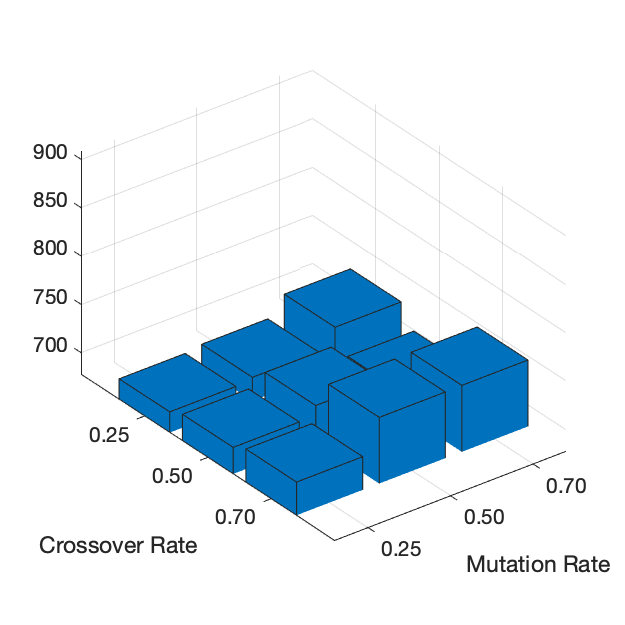
\includegraphics[width=0.5\textwidth]{crossover/min/cross_alt_edges_1.png}
		\caption{Alternating Edges Crossover (adjacency representation)}
		\label{fig:z}
    	\end{subfigure}\\
%
	\begin{subfigure}[b]{0.25\textwidth}
		\centering
		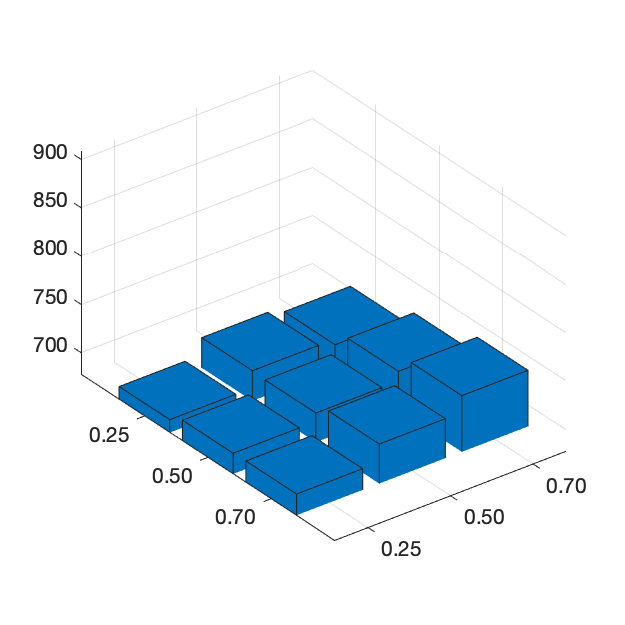
\includegraphics[width=0.9\textwidth]{crossover/min/cross_cycle_1.png}
		\caption{\texttt{CX}}
		\label{fig:x}
    	\end{subfigure}
%
	\begin{subfigure}[b]{0.25\textwidth}
		\centering
		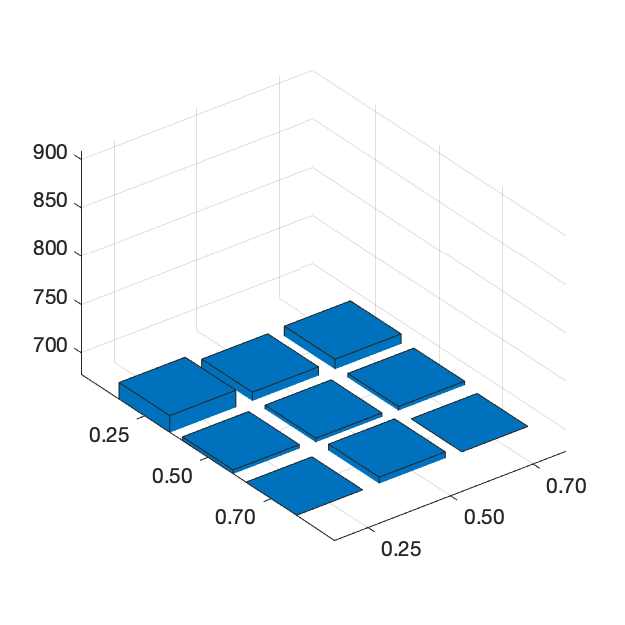
\includegraphics[width=0.9\textwidth]{crossover/min/cross_edge_heuristic_1.png}
		\caption{\texttt{HERX}}
		\label{fig:y}
    	\end{subfigure}
%
	\begin{subfigure}[b]{0.25\textwidth}
		\centering
		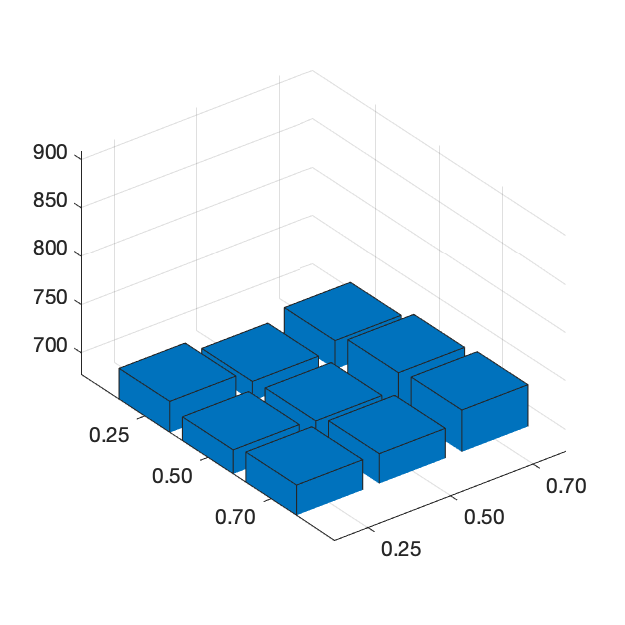
\includegraphics[width=0.9\textwidth]{crossover/min/cross_edge_recombination_1.png}
		\caption{\texttt{ERX}}
		\label{fig:z}
    	\end{subfigure}
%
	\begin{subfigure}[b]{0.25\textwidth}
		\centering
		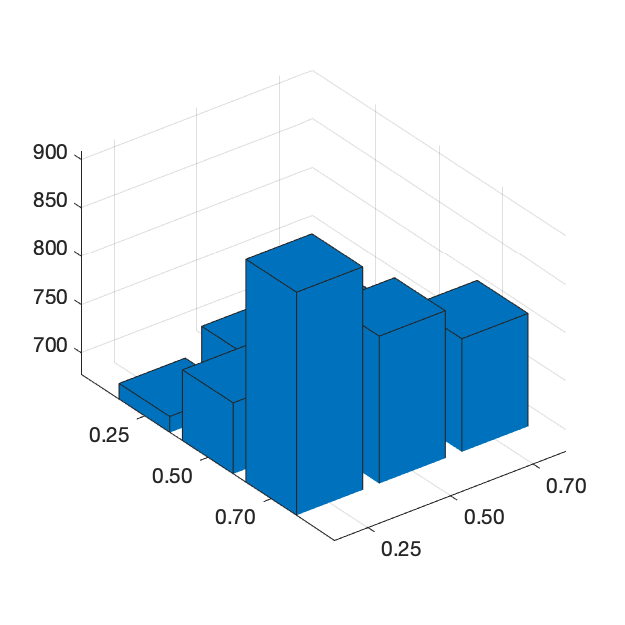
\includegraphics[width=0.9\textwidth]{crossover/min/cross_heuristic_1.png}
		\caption{\texttt{HEUR}}
		\label{fig:x}
    	\end{subfigure}
%
	\begin{subfigure}[b]{0.25\textwidth}
		\centering
		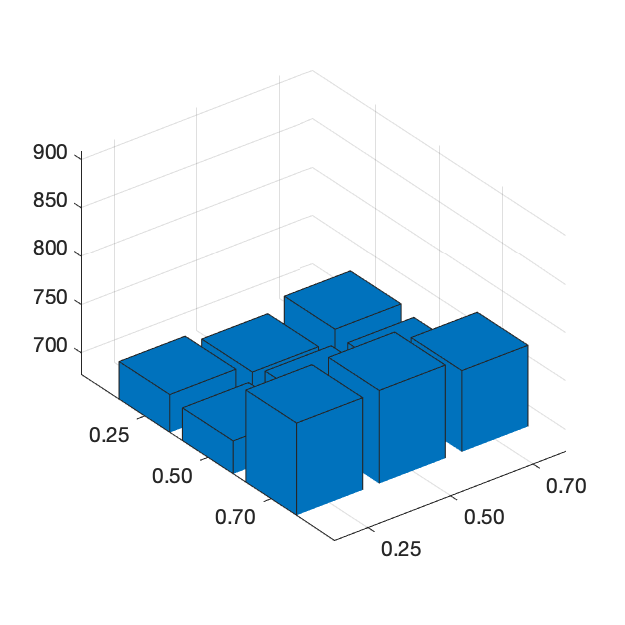
\includegraphics[width=0.9\textwidth]{crossover/min/cross_max_preservative_1.png}
		\caption{\texttt{MPX}}
		\label{fig:y}
    	\end{subfigure}
%
	\begin{subfigure}[b]{0.25\textwidth}
		\centering
		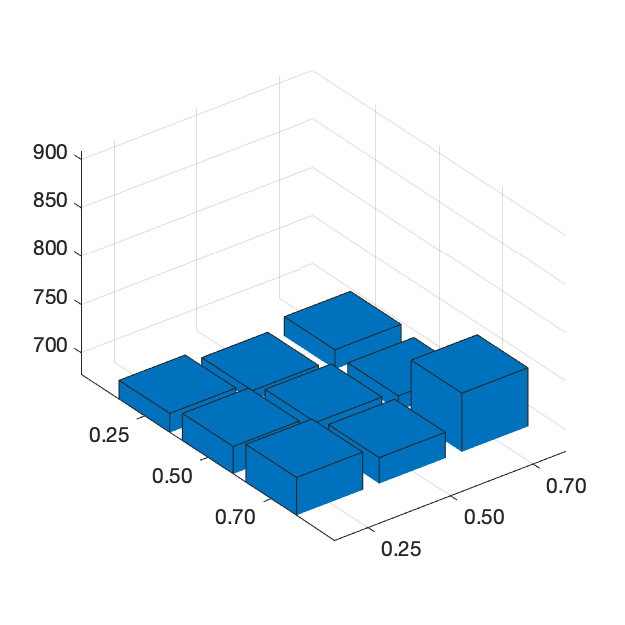
\includegraphics[width=0.9\textwidth]{crossover/min/cross_order_1.png}
		\caption{\texttt{O1}}
		\label{fig:z}
    	\end{subfigure}
%
	\begin{subfigure}[b]{0.25\textwidth}
		\centering
		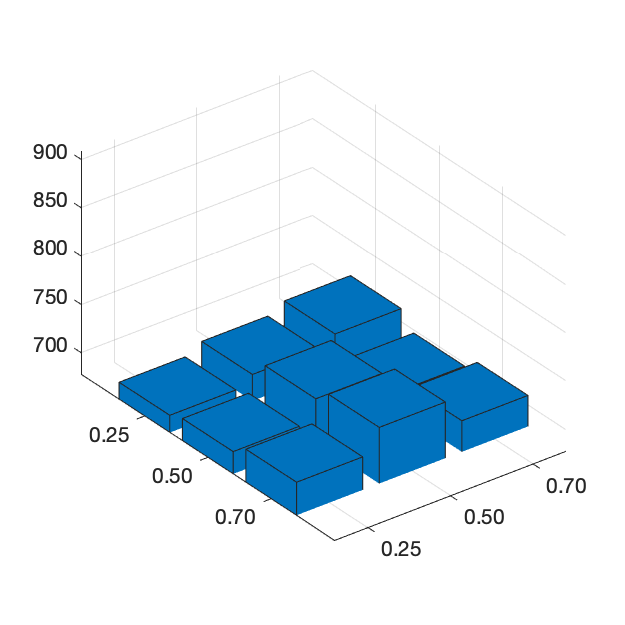
\includegraphics[width=0.9\textwidth]{crossover/min/cross_order_based_1.png}
		\caption{\texttt{O2}}
		\label{fig:x}
    	\end{subfigure}
%
	\begin{subfigure}[b]{0.25\textwidth}
		\centering
		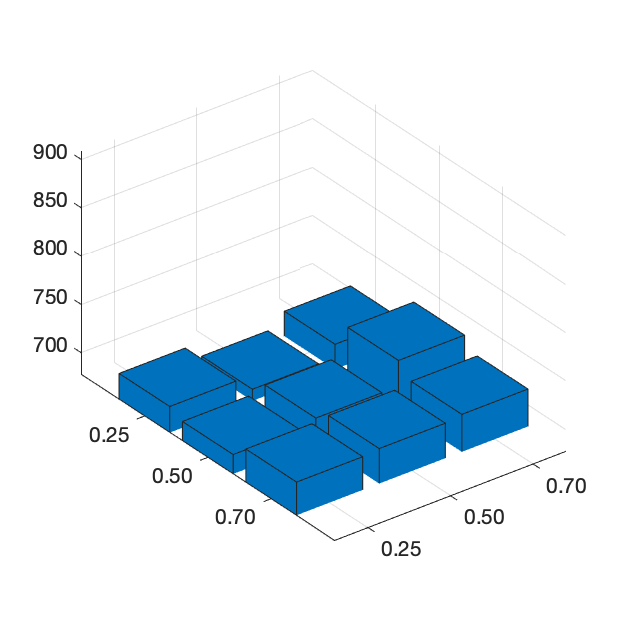
\includegraphics[width=0.9\textwidth]{crossover/min/cross_sp_1.png}
		\caption{\texttt{XOVSP}}
		\label{fig:y}
    	\end{subfigure}
%
	\begin{subfigure}[b]{0.25\textwidth}
		\centering
		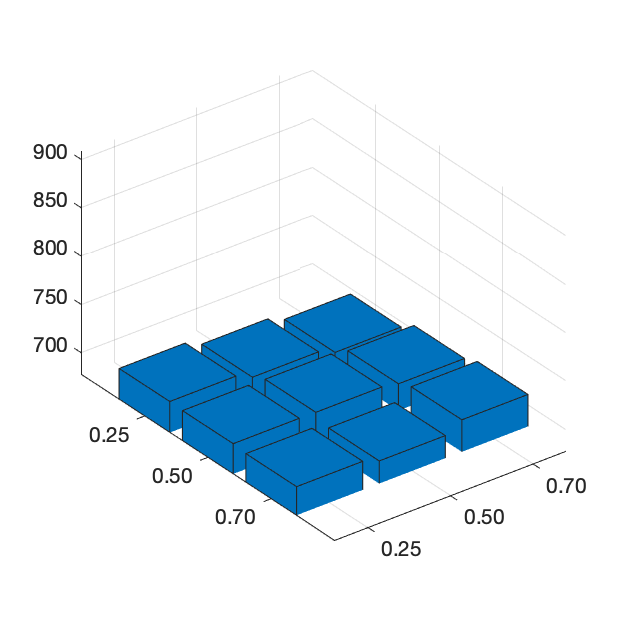
\includegraphics[width=0.9\textwidth]{crossover/min/cross_partial_map_1.png}
		\caption{\texttt{PMX}}
		\label{fig:z}
    	\end{subfigure}
%
	\begin{subfigure}[b]{0.25\textwidth}
		\centering
		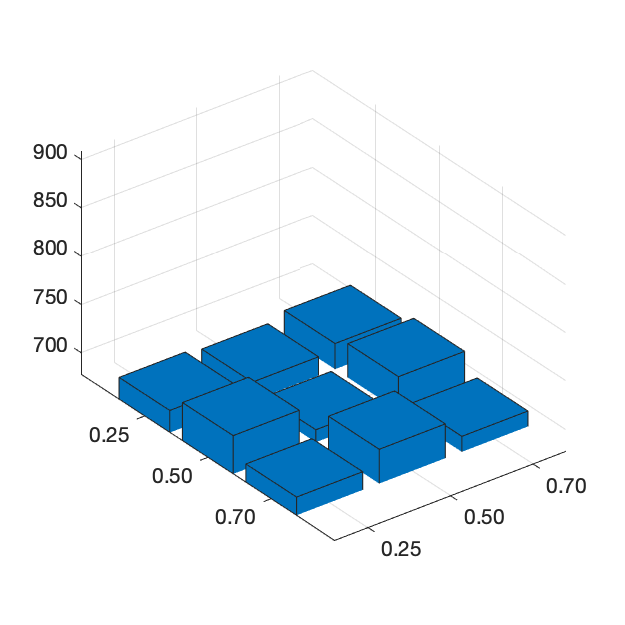
\includegraphics[width=0.9\textwidth]{crossover/min/cross_position_based_1.png}
		\caption{\texttt{POS}}
		\label{fig:x}
    	\end{subfigure}
%
	\begin{subfigure}[b]{0.25\textwidth}
		\centering
		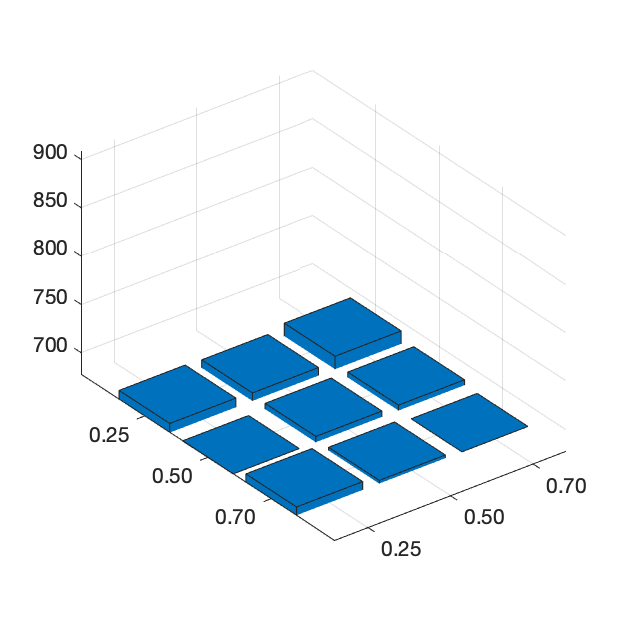
\includegraphics[width=0.9\textwidth]{crossover/min/cross_seq_constructive_1.png}
		\caption{\texttt{SCX}}
		\label{fig:y}
    	\end{subfigure}
%
	\begin{subfigure}[b]{0.25\textwidth}
		\centering
		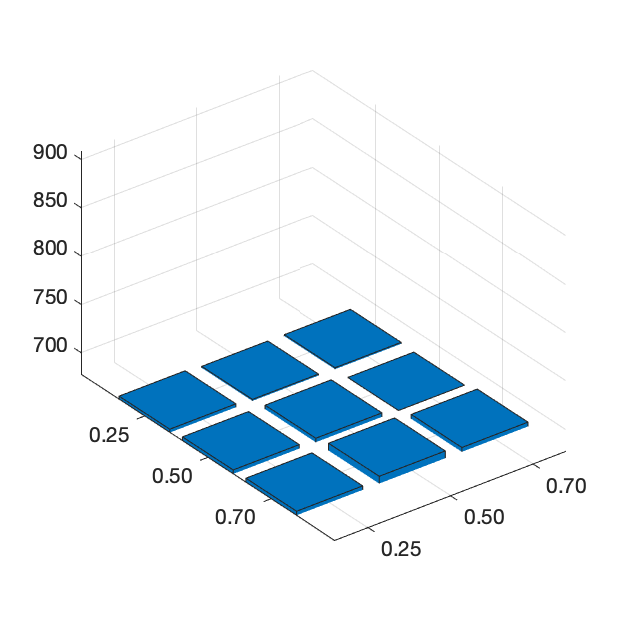
\includegraphics[width=0.9\textwidth]{crossover/min/cross_unnamed_1.png}
		\caption{\texttt{UHX}}
		\label{fig:z}
    	\end{subfigure}
	\caption{Shortest tour found by each crossover operator (tour of 70 cities). Maximum of 1000 generations and basic stopping criterion (the algorithm stops when there has been no improvement in 100 generations which is quite strict, such that late and surprising improvements can be ruled out). The stop condition was met in most cases.}
	\label{fig:rescross1}
\end{figure}

%%%%%%%%%%%%%%%%%%%%%%%%%%%%%%%%%%%%%%%%%%%%%%%%%%%%%%%%%%%%%%%%%%%%%%%%%%%%%%%%%%%%%%%%%%%%%%%%%%%%%%%%%
%%%%%%%%%%%%%%%%%%%%%%%%%%%%%%%%%%%%%%%%%%%%%%%%%%%%%%%%%%%%%%%%%%%%%%%%%%%%%%%%%%%%%%%%%%%%%%%%%%%%%%%%%
%%%%%%%%%%%%%%%%%%%%%%%%%%%%%%%%%%%%%%%%%%%%%%%%%%%%%%%%%%%%%%%%%%%%%%%%%%%%%%%%%%%%%%%%%%%%%%%%%%%%%%%%%

\pagenumbering{gobble}
\begin{figure}[H]
	\centering
%
	\begin{subfigure}[b]{0.7\textwidth}
		\centering
		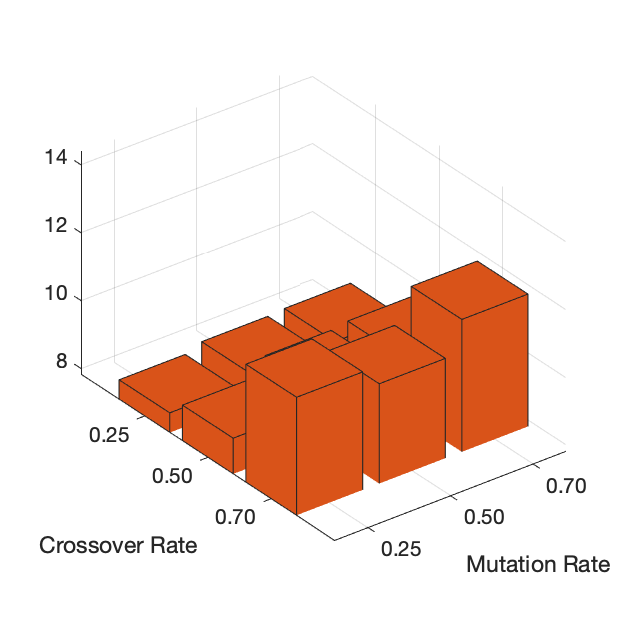
\includegraphics[width=0.5\textwidth]{crossover/min/cross_alt_edges_2.png}
		\caption{Alternating Edges Crossover (adjacency representation)}
		\label{fig:z}
    	\end{subfigure}\\
%
	\begin{subfigure}[b]{0.25\textwidth}
		\centering
		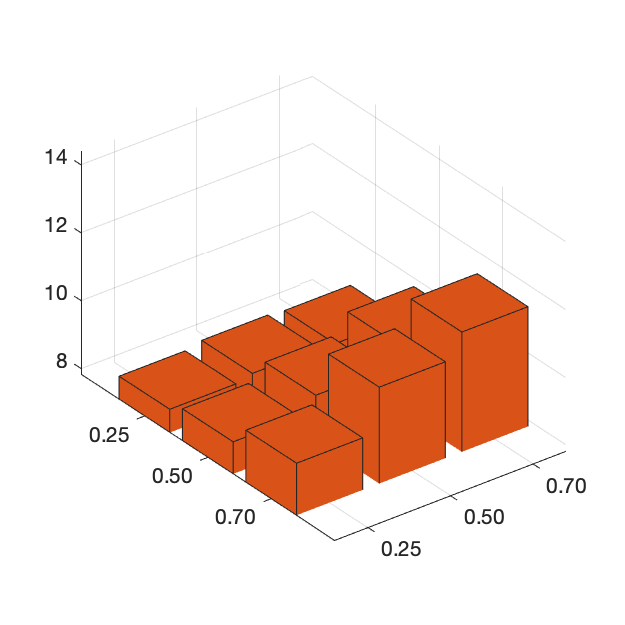
\includegraphics[width=0.9\textwidth]{crossover/min/cross_cycle_2.png}
		\caption{\texttt{CX}}
		\label{fig:x}
    	\end{subfigure}
%
	\begin{subfigure}[b]{0.25\textwidth}
		\centering
		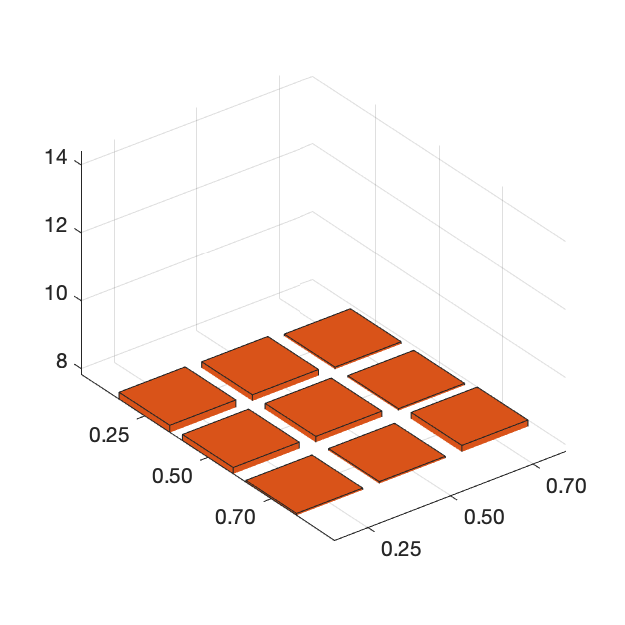
\includegraphics[width=0.9\textwidth]{crossover/min/cross_edge_heuristic_2.png}
		\caption{\texttt{HERX}}
		\label{fig:y}
    	\end{subfigure}
%
	\begin{subfigure}[b]{0.25\textwidth}
		\centering
		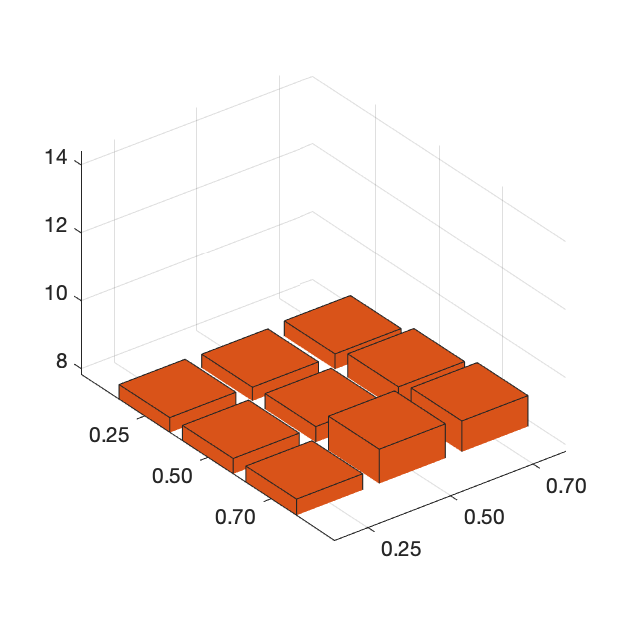
\includegraphics[width=0.9\textwidth]{crossover/min/cross_edge_recombination_2.png}
		\caption{\texttt{ERX}}
		\label{fig:z}
    	\end{subfigure}
%
	\begin{subfigure}[b]{0.25\textwidth}
		\centering
		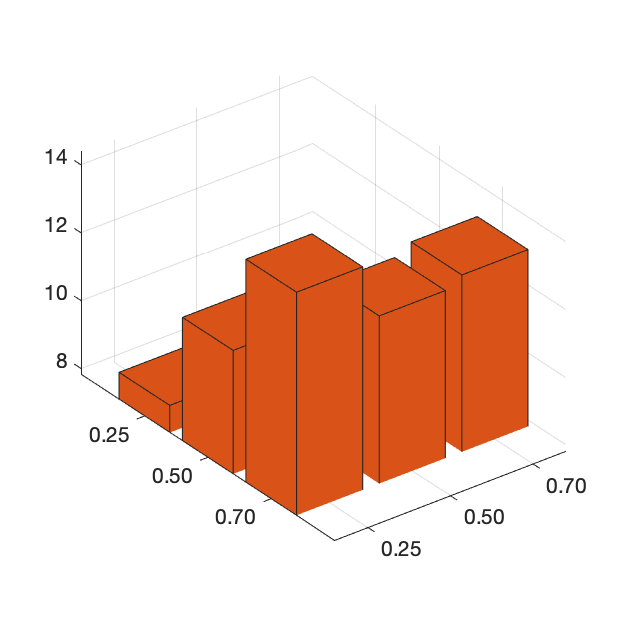
\includegraphics[width=0.9\textwidth]{crossover/min/cross_heuristic_2.png}
		\caption{\texttt{HEUR}}
		\label{fig:x}
    	\end{subfigure}
%
	\begin{subfigure}[b]{0.25\textwidth}
		\centering
		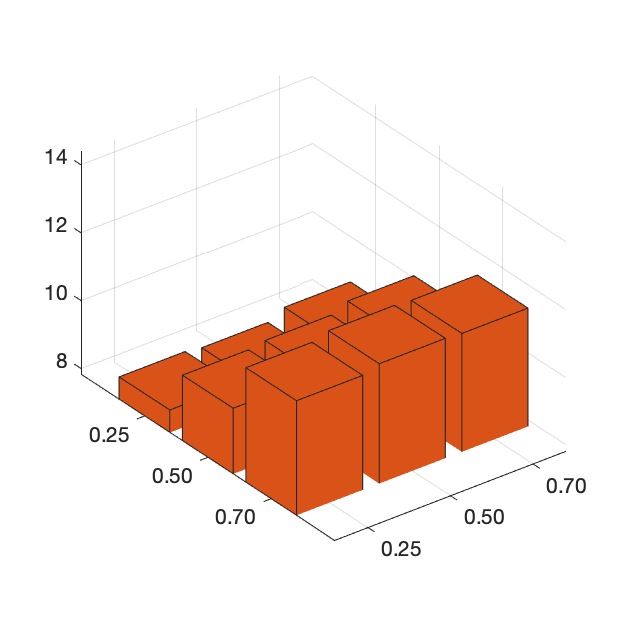
\includegraphics[width=0.9\textwidth]{crossover/min/cross_max_preservative_2.png}
		\caption{\texttt{MPX}}
		\label{fig:y}
    	\end{subfigure}
%
	\begin{subfigure}[b]{0.25\textwidth}
		\centering
		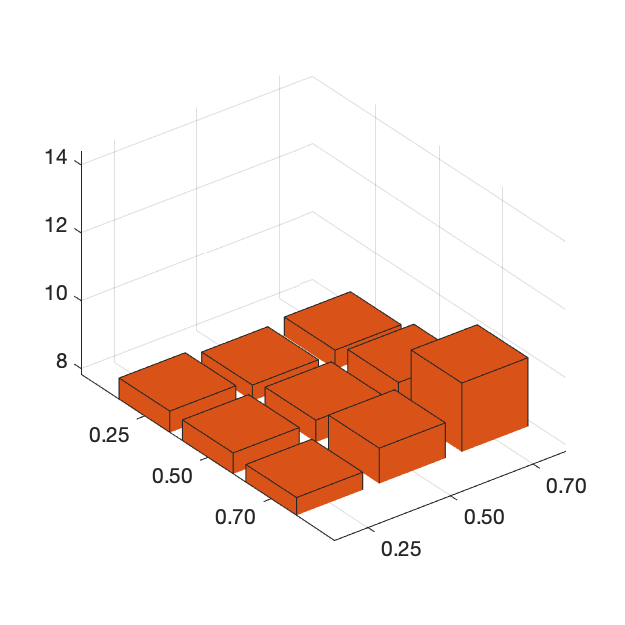
\includegraphics[width=0.9\textwidth]{crossover/min/cross_order_2.png}
		\caption{\texttt{O1}}
		\label{fig:z}
    	\end{subfigure}
%
	\begin{subfigure}[b]{0.25\textwidth}
		\centering
		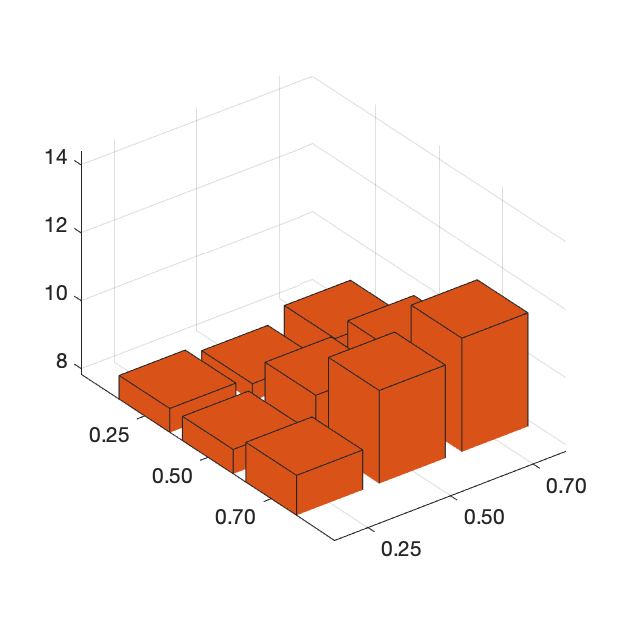
\includegraphics[width=0.9\textwidth]{crossover/min/cross_order_based_2.png}
		\caption{\texttt{O2}}
		\label{fig:x}
    	\end{subfigure}
%
	\begin{subfigure}[b]{0.25\textwidth}
		\centering
		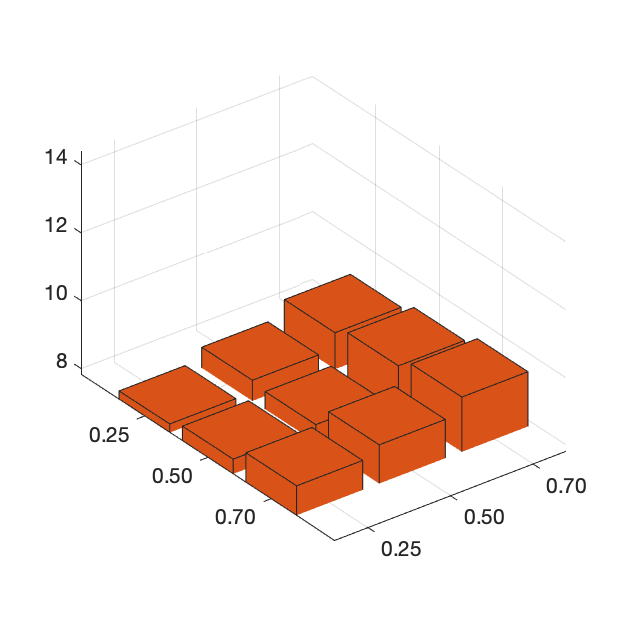
\includegraphics[width=0.9\textwidth]{crossover/min/cross_sp_2.png}
		\caption{\texttt{XOVSP}}
		\label{fig:y}
    	\end{subfigure}
%
	\begin{subfigure}[b]{0.25\textwidth}
		\centering
		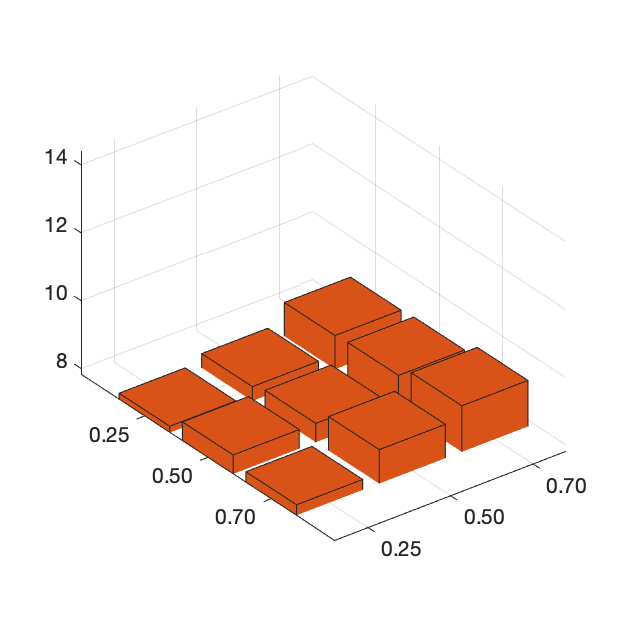
\includegraphics[width=0.9\textwidth]{crossover/min/cross_partial_map_2.png}
		\caption{\texttt{PMX}}
		\label{fig:z}
    	\end{subfigure}
%
	\begin{subfigure}[b]{0.25\textwidth}
		\centering
		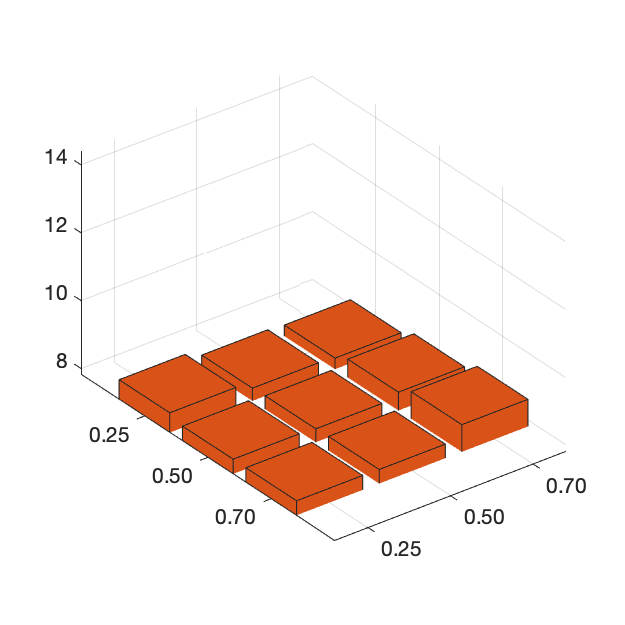
\includegraphics[width=0.9\textwidth]{crossover/min/cross_position_based_2.png}
		\caption{\texttt{POS}}
		\label{fig:x}
    	\end{subfigure}
%
	\begin{subfigure}[b]{0.25\textwidth}
		\centering
		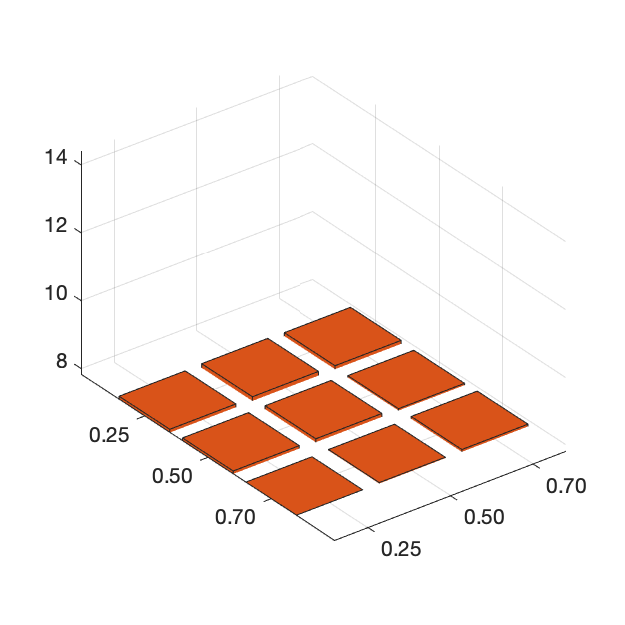
\includegraphics[width=0.9\textwidth]{crossover/min/cross_seq_constructive_2.png}
		\caption{\texttt{SCX}}
		\label{fig:y}
    	\end{subfigure}
%
	\begin{subfigure}[b]{0.25\textwidth}
		\centering
		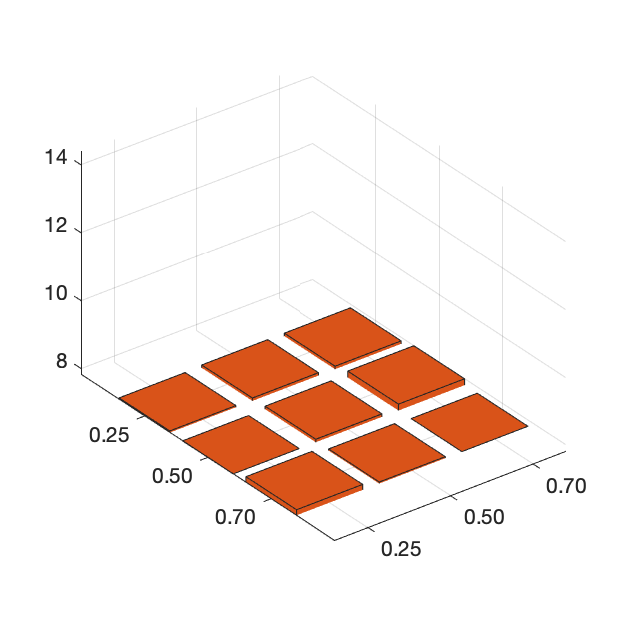
\includegraphics[width=0.9\textwidth]{crossover/min/cross_unnamed_2.png}
		\caption{\texttt{UHX}}
		\label{fig:z}
    	\end{subfigure}
	\caption{Shortest tour found by each crossover operator (tour of 100 cities). Maximum of 1000 generations and basic stopping criterion (the algorithm stops when there has been no improvement in 100 generations which is quite strict, such that late and surprising improvements can be ruled out). The stop condition was met in most cases.}
	\label{fig:rescross2}
\end{figure}

%%%%%%%%%%%%%%%%%%%%%%%%%%%%%%%%%%%%%%%%%%%%%%%%%%%%%%%%%%%%%%%%%%%%%%%%%%%%%%%%%%%%%%%%%%%%%%%%%%%%%%%%%
%%%%%%%%%%%%%%%%%%%%%%%%%%%%%%%%%%%%%%%%%%%%%%%%%%%%%%%%%%%%%%%%%%%%%%%%%%%%%%%%%%%%%%%%%%%%%%%%%%%%%%%%%
%%%%%%%%%%%%%%%%%%%%%%%%%%%%%%%%%%%%%%%%%%%%%%%%%%%%%%%%%%%%%%%%%%%%%%%%%%%%%%%%%%%%%%%%%%%%%%%%%%%%%%%%%

\pagenumbering{gobble}
\begin{figure}[H]
	\centering
%
	\begin{subfigure}[b]{0.7\textwidth}
		\centering
		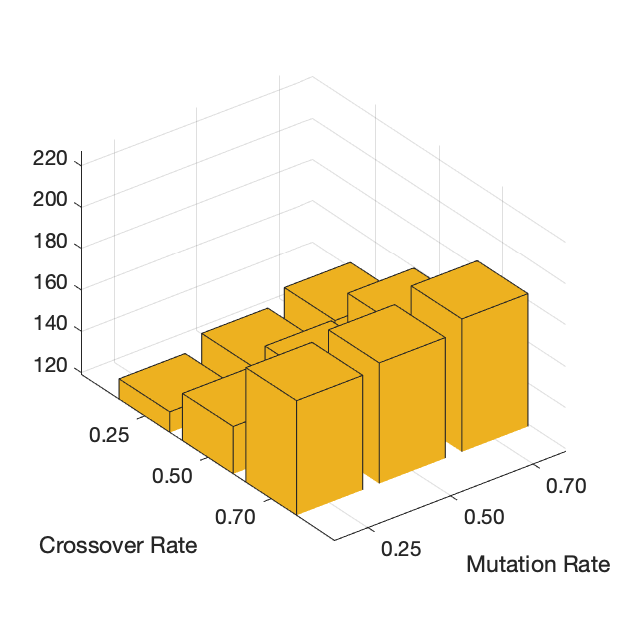
\includegraphics[width=0.5\textwidth]{crossover/min/cross_alt_edges_3.png}
		\caption{Alternating Edges Crossover (adjacency representation)}
		\label{fig:z}
    	\end{subfigure}\\
%
	\begin{subfigure}[b]{0.25\textwidth}
		\centering
		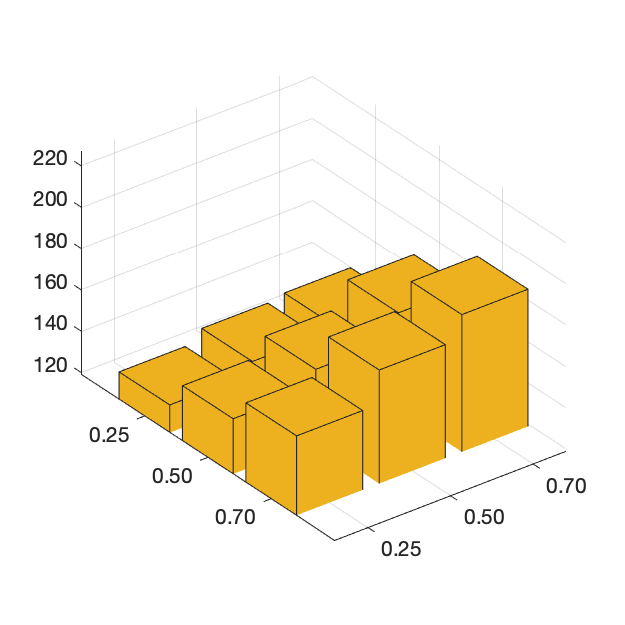
\includegraphics[width=0.9\textwidth]{crossover/min/cross_cycle_3.png}
		\caption{\texttt{CX}}
		\label{fig:x}
    	\end{subfigure}
%
	\begin{subfigure}[b]{0.25\textwidth}
		\centering
		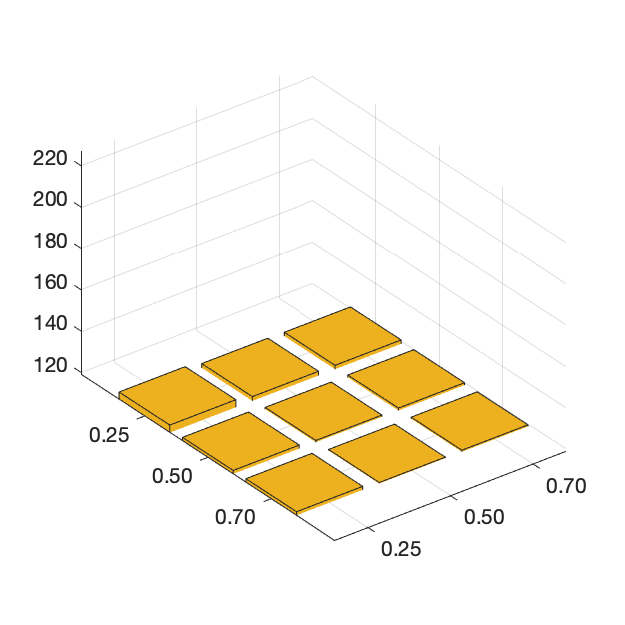
\includegraphics[width=0.9\textwidth]{crossover/min/cross_edge_heuristic_3.png}
		\caption{\texttt{HERX}}
		\label{fig:y}
    	\end{subfigure}
%
	\begin{subfigure}[b]{0.25\textwidth}
		\centering
		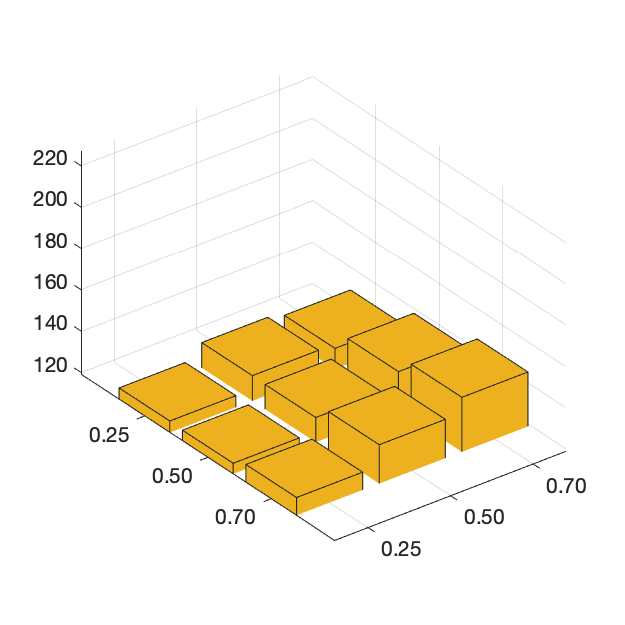
\includegraphics[width=0.9\textwidth]{crossover/min/cross_edge_recombination_3.png}
		\caption{\texttt{ERX}}
		\label{fig:z}
    	\end{subfigure}
%
	\begin{subfigure}[b]{0.25\textwidth}
		\centering
		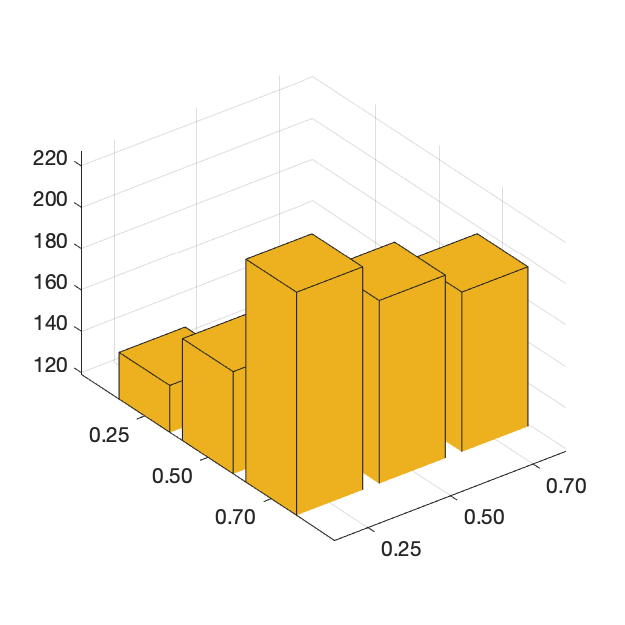
\includegraphics[width=0.9\textwidth]{crossover/min/cross_heuristic_3.png}
		\caption{\texttt{HEUR}}
		\label{fig:x}
    	\end{subfigure}
%
	\begin{subfigure}[b]{0.25\textwidth}
		\centering
		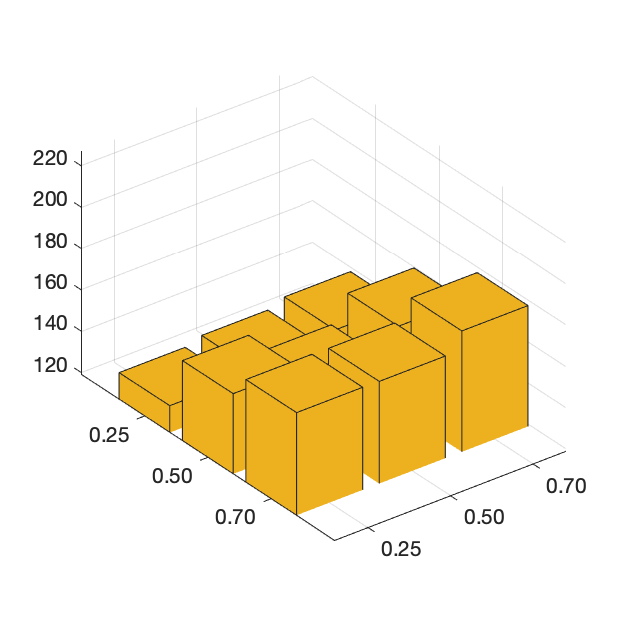
\includegraphics[width=0.9\textwidth]{crossover/min/cross_max_preservative_3.png}
		\caption{\texttt{MPX}}
		\label{fig:y}
    	\end{subfigure}
%
	\begin{subfigure}[b]{0.25\textwidth}
		\centering
		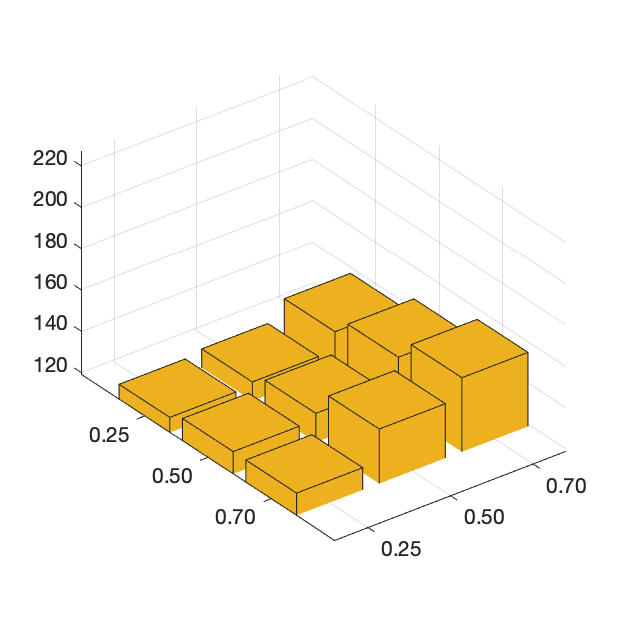
\includegraphics[width=0.9\textwidth]{crossover/min/cross_order_3.png}
		\caption{\texttt{O1}}
		\label{fig:z}
    	\end{subfigure}
%
	\begin{subfigure}[b]{0.25\textwidth}
		\centering
		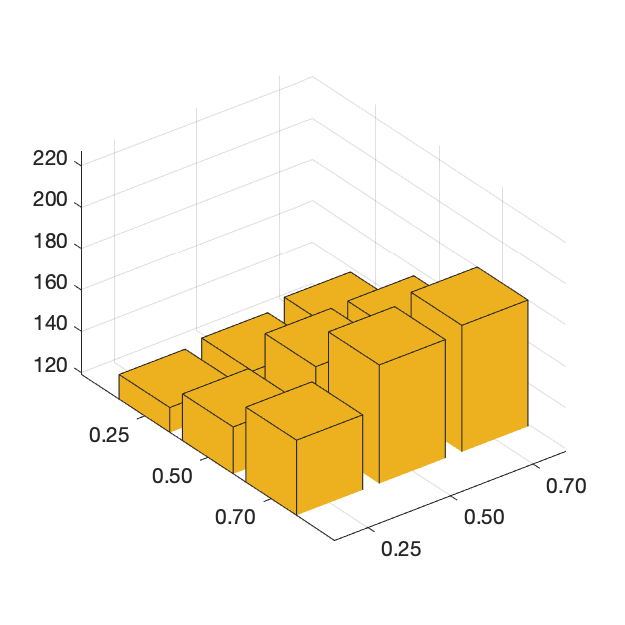
\includegraphics[width=0.9\textwidth]{crossover/min/cross_order_based_3.png}
		\caption{\texttt{O2}}
		\label{fig:x}
    	\end{subfigure}
%
	\begin{subfigure}[b]{0.25\textwidth}
		\centering
		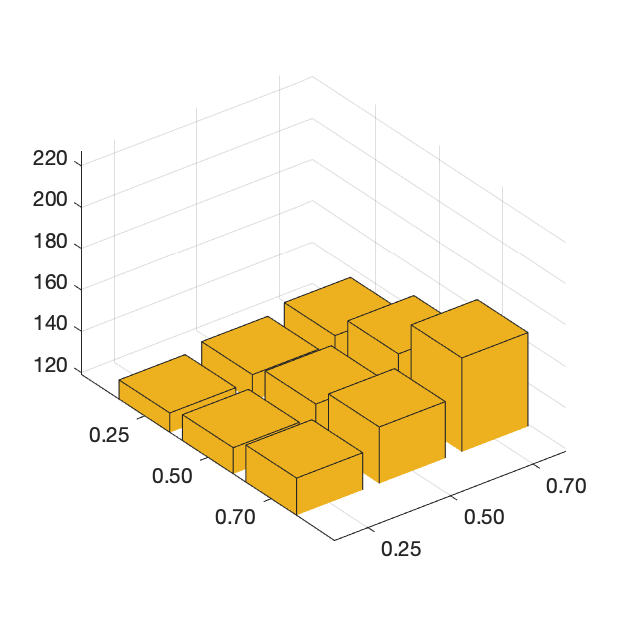
\includegraphics[width=0.9\textwidth]{crossover/min/cross_sp_3.png}
		\caption{\texttt{XOVSP}}
		\label{fig:y}
    	\end{subfigure}
%
	\begin{subfigure}[b]{0.25\textwidth}
		\centering
		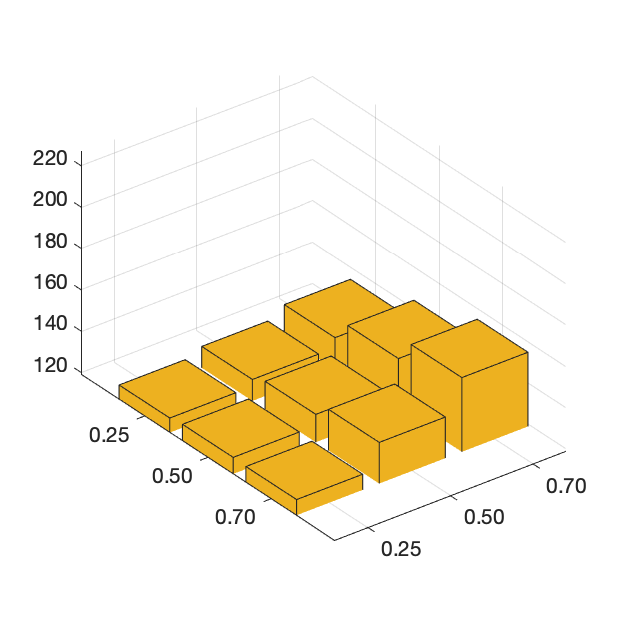
\includegraphics[width=0.9\textwidth]{crossover/min/cross_partial_map_3.png}
		\caption{\texttt{PMX}}
		\label{fig:z}
    	\end{subfigure}
%
	\begin{subfigure}[b]{0.25\textwidth}
		\centering
		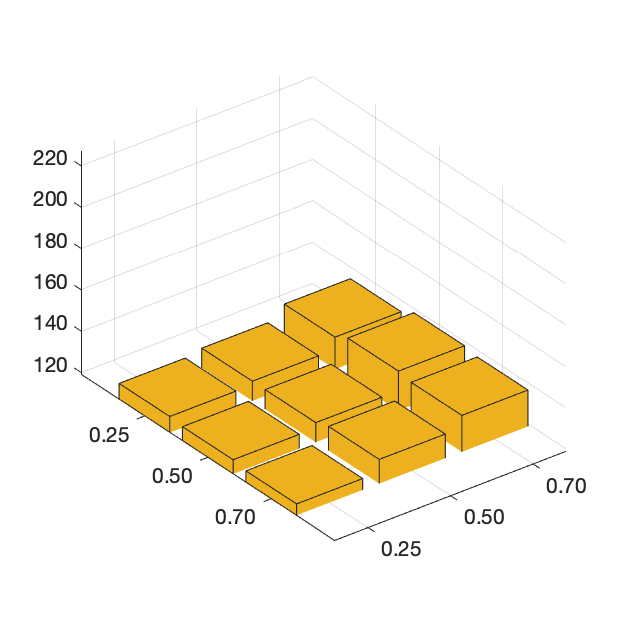
\includegraphics[width=0.9\textwidth]{crossover/min/cross_position_based_3.png}
		\caption{\texttt{POS}}
		\label{fig:x}
    	\end{subfigure}
%
	\begin{subfigure}[b]{0.25\textwidth}
		\centering
		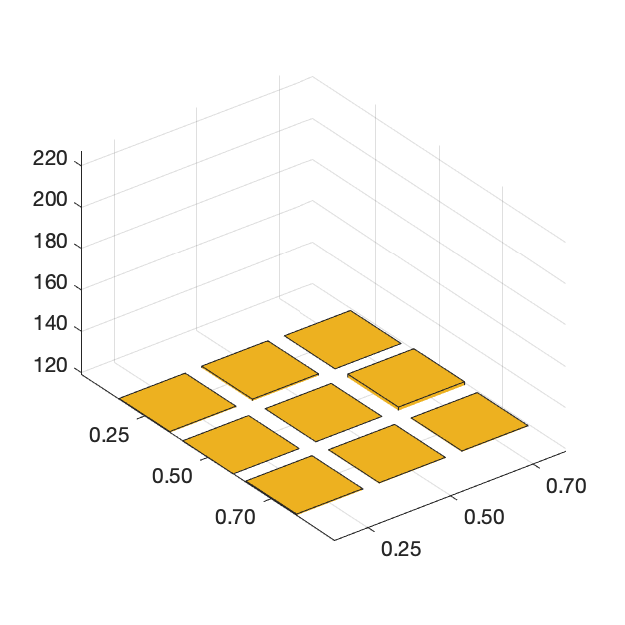
\includegraphics[width=0.9\textwidth]{crossover/min/cross_seq_constructive_3.png}
		\caption{\texttt{SCX}}
		\label{fig:y}
    	\end{subfigure}
%
	\begin{subfigure}[b]{0.25\textwidth}
		\centering
		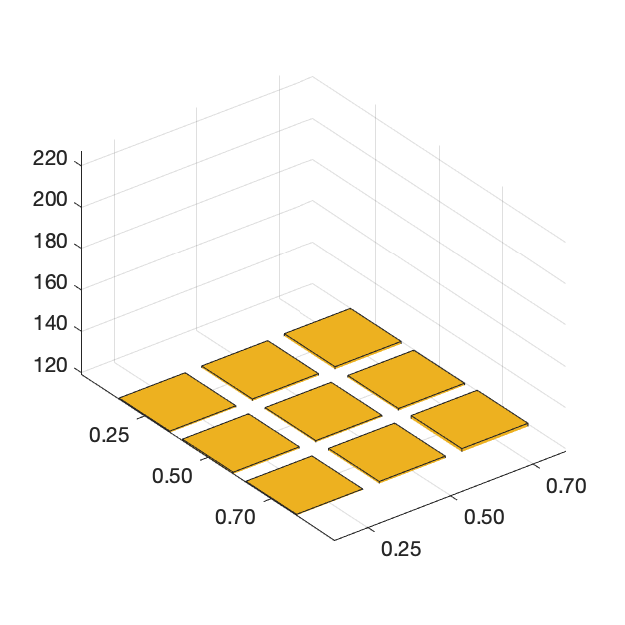
\includegraphics[width=0.9\textwidth]{crossover/min/cross_unnamed_3.png}
		\caption{\texttt{UHX}}
		\label{fig:z}
    	\end{subfigure}
	\caption{Shortest tour found by each crossover operator (tour of 127 cities). Maximum of 1000 generations and basic stopping criterion (the algorithm stops when there has been no improvement in 100 generations which is quite strict, such that late and surprising improvements can be ruled out). The stop condition was met in most cases.}
	\label{fig:rescross3}
\end{figure}

%%%%%%%%%%%%%%%%%%%%%%%%%%%%%%%%%%%%%%%%%%%%%%%%%%%%%%%%%%%%%%%%%%%%%%%%%%%%%%%%%%%%%%%%%%%%%%%%%%%%%%%%%
%%%%%%%%%%%%%%%%%%%%%%%%%%%%%%%%%%%%%%%%%%%%%%%%%%%%%%%%%%%%%%%%%%%%%%%%%%%%%%%%%%%%%%%%%%%%%%%%%%%%%%%%%
%%%%%%%%%%%%%%%%%%%%%%%%%%%%%%%%%%%%%%%%%%%%%%%%%%%%%%%%%%%%%%%%%%%%%%%%%%%%%%%%%%%%%%%%%%%%%%%%%%%%%%%%%

\pagenumbering{gobble}
\begin{figure}[H]
	\centering
%
	\begin{subfigure}[b]{0.7\textwidth}
		\centering
		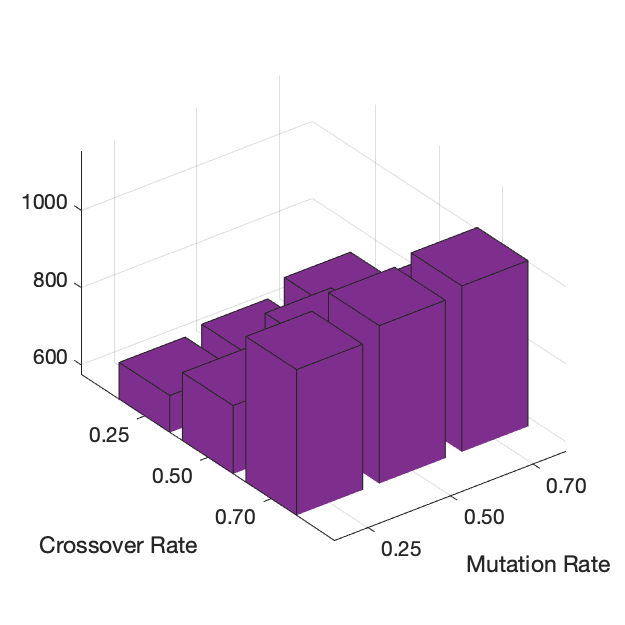
\includegraphics[width=0.5\textwidth]{crossover/min/cross_alt_edges_4.png}
		\caption{Alternating Edges Crossover (adjacency representation)}
		\label{fig:z}
    	\end{subfigure}\\
%
	\begin{subfigure}[b]{0.25\textwidth}
		\centering
		\includegraphics[width=0.9\textwidth]{crossover/min/cross_cycle_4.png}
		\caption{\texttt{CX}}
		\label{fig:x}
    	\end{subfigure}
%
	\begin{subfigure}[b]{0.25\textwidth}
		\centering
		\includegraphics[width=0.9\textwidth]{crossover/min/cross_edge_heuristic_4.png}
		\caption{\texttt{HERX}}
		\label{fig:y}
    	\end{subfigure}
%
	\begin{subfigure}[b]{0.25\textwidth}
		\centering
		\includegraphics[width=0.9\textwidth]{crossover/min/cross_edge_recombination_4.png}
		\caption{\texttt{ERX}}
		\label{fig:z}
    	\end{subfigure}
%
	\begin{subfigure}[b]{0.25\textwidth}
		\centering
		\includegraphics[width=0.9\textwidth]{crossover/min/cross_heuristic_4.png}
		\caption{\texttt{HEUR}}
		\label{fig:x}
    	\end{subfigure}
%
	\begin{subfigure}[b]{0.25\textwidth}
		\centering
		\includegraphics[width=0.9\textwidth]{crossover/min/cross_max_preservative_4.png}
		\caption{\texttt{MPX}}
		\label{fig:y}
    	\end{subfigure}
%
	\begin{subfigure}[b]{0.25\textwidth}
		\centering
		\includegraphics[width=0.9\textwidth]{crossover/min/cross_order_4.png}
		\caption{\texttt{O1}}
		\label{fig:z}
    	\end{subfigure}
%
	\begin{subfigure}[b]{0.25\textwidth}
		\centering
		\includegraphics[width=0.9\textwidth]{crossover/min/cross_order_based_4.png}
		\caption{\texttt{O2}}
		\label{fig:x}
    	\end{subfigure}
%
	\begin{subfigure}[b]{0.25\textwidth}
		\centering
		\includegraphics[width=0.9\textwidth]{crossover/min/cross_sp_4.png}
		\caption{\texttt{XOVSP}}
		\label{fig:y}
    	\end{subfigure}
%
	\begin{subfigure}[b]{0.25\textwidth}
		\centering
		\includegraphics[width=0.9\textwidth]{crossover/min/cross_partial_map_4.png}
		\caption{\texttt{PMX}}
		\label{fig:z}
    	\end{subfigure}
%
	\begin{subfigure}[b]{0.25\textwidth}
		\centering
		\includegraphics[width=0.9\textwidth]{crossover/min/cross_position_based_4.png}
		\caption{\texttt{POS}}
		\label{fig:x}
    	\end{subfigure}
%
	\begin{subfigure}[b]{0.25\textwidth}
		\centering
		\includegraphics[width=0.9\textwidth]{crossover/min/cross_seq_constructive_4.png}
		\caption{\texttt{SCX}}
		\label{fig:y}
    	\end{subfigure}
%
	\begin{subfigure}[b]{0.25\textwidth}
		\centering
		\includegraphics[width=0.9\textwidth]{crossover/min/cross_unnamed_4.png}
		\caption{\texttt{UHX}}
		\label{fig:z}
    	\end{subfigure}
	\caption{Shortest tour found by each crossover operator (tour of 131 cities). Maximum of 1000 generations and basic stopping criterion (the algorithm stops when there has been no improvement in 100 generations which is quite strict, such that late and surprising improvements can be ruled out). The stop condition was met in most cases.}
	\label{fig:rescross4}
\end{figure}

%\restoregeometry
\advance\voffset by 0.6cm



